\documentclass[iop, tighten]{emulateapj}
%\documentclass[12pt,preprint]{aastex}

\usepackage{amsmath}
\usepackage[draft]{hyperref}  % draft suppresses all hyperlinks except urls

% Math macros
% -----------
% Units
\newcommand{\msun}{\ensuremath{\,M_\odot}}
\newcommand{\ssec}{\ensuremath{\,\mathrm{s}}}
\newcommand{\yr}{\ensuremath{\,\mathrm{yr}}}
\newcommand{\myr}{\ensuremath{\,\mathrm{Myr}}}
\newcommand{\erg}{\ensuremath{\,\mathrm{erg}}}
\newcommand{\cm}{\ensuremath{\,\mathrm{cm}}}
\newcommand{\pc}{\ensuremath{\,\mathrm{pc}}}
\newcommand{\kpc}{\ensuremath{\,\mathrm{kpc}}}
\newcommand{\dex}{\ensuremath{\,\mathrm{dex}}}
\newcommand{\ang}{\ensuremath{\,\textrm{\AA}}}
\newcommand{\ddeg}{\ensuremath{\,\mathrm{deg}}}
\newcommand{\aarcsec}{\ensuremath{\,\mathrm{arcsec}}}
\newcommand{\uflambda}{\ensuremath{\, \erg\ssec^{-1}\cm^{-2}\ang^{-1}}}


% Filters
\newcommand{\filter}{\ensuremath{\mathrm{X}}}  % Arbitrary filter
\newcommand{\fuv}{\ensuremath{\mathrm{FUV}}}
\newcommand{\nuv}{\ensuremath{\mathrm{NUV}}}
\newcommand{\acsb}{\ensuremath{\mathrm{F475W}}}
\newcommand{\acsi}{\ensuremath{\mathrm{F814W}}}


% Basic quantities
\newcommand{\sfh}{\ensuremath{\mathrm{SFH}}}
\newcommand{\sfr}{\ensuremath{\mathrm{SFR}}}
\newcommand{\meansfr}{\ensuremath{\langle\sfr\rangle}}

\newcommand{\met}{\ensuremath{\mathrm{[M/H]}}}

\newcommand{\avf}{\ensuremath{A_{\mathrm{V}f}}}
\newcommand{\dav}{\ensuremath{dA_\mathrm{V}}}
\newcommand{\ax}{\ensuremath{A_\filter}}
\newcommand{\afuv}{\ensuremath{A_\fuv}}
\newcommand{\anuv}{\ensuremath{A_\nuv}}
\newcommand{\rv}{\ensuremath{R_\mathrm{V}}}


% Words
\newcommand{\obs}{\ensuremath{\mathrm{obs}}}


% Specific quantities
\newcommand{\xobs}{\ensuremath{m_{\filter,\obs}}}  % Observed mag
\newcommand{\fuvobs}{\ensuremath{m_\fuv^\obs}}
\newcommand{\nuvobs}{\ensuremath{m_\nuv^\obs}}
\newcommand{\xsfh}{\ensuremath{m_\filter^\sfh}}  % Modeled attenuated mag
\newcommand{\fuvsfh}{\ensuremath{m_\fuv^\sfh}}
\newcommand{\nuvsfh}{\ensuremath{m_\nuv^\sfh}}
\newcommand{\xsfhz}{\ensuremath{m_\filter^{\sfh,0}}}  % Modeled intrinsic mag
\newcommand{\fuvsfhz}{\ensuremath{m_\fuv^{\sfh,0}}}
\newcommand{\nuvsfhz}{\ensuremath{m_\nuv^{\sfh,0}}}
\newcommand{\fuvnuvobs}{\ensuremath{(m_\fuv-m_\nuv)^\obs}}
\newcommand{\fuvnuvsfh}{\ensuremath{(m_\fuv-m_\nuv)^\sfh}}
\newcommand{\fuvnuvsfhz}{\ensuremath{(m_\fuv-m_\nuv)^{\sfh,0}}}

\newcommand{\fxobs}{\ensuremath{f_\filter^\obs}}  % Observed flux
\newcommand{\ffuvobs}{\ensuremath{f_\fuv^\obs}}
\newcommand{\fnuvobs}{\ensuremath{f_\nuv^\obs}}
\newcommand{\fxsfh}{\ensuremath{f_\filter^\sfh}}  % Modeled attenuated flux
\newcommand{\ffuvsfh}{\ensuremath{f_\fuv^\sfh}}
\newcommand{\fnuvsfh}{\ensuremath{f_\nuv^\sfh}}
\newcommand{\fxsfhz}{\ensuremath{f_\filter^{\sfh,0}}}  % Modeled intrinsic flux
\newcommand{\ffuvsfhz}{\ensuremath{f_\fuv^{\sfh,0}}}
\newcommand{\fnuvsfhz}{\ensuremath{f_\nuv^{\sfh,0}}}

\newcommand{\sfrx}{\ensuremath{\sfr_\filter}}  % Observed flux-based SFR
\newcommand{\sfrfuv}{\ensuremath{\sfr_\fuv}}
\newcommand{\sfrnuv}{\ensuremath{\sfr_\nuv}}
\newcommand{\sfrxz}{\ensuremath{\sfr_\filter^0}}  % Modeled flux-based SFR
\newcommand{\sfrfuvz}{\ensuremath{\sfr_\fuv^0}}
\newcommand{\sfrnuvz}{\ensuremath{\sfr_\nuv^0}}
\newcommand{\sfroneh}{\ensuremath{\meansfr_{100}}}  % 100-Myr mean SFR from SFH

\newcommand{\lx}{\ensuremath{L_\filter}}  % Luminosity
\newcommand{\lfuv}{\ensuremath{L_\fuv}}
\newcommand{\lnuv}{\ensuremath{L_\nuv}}


% Other
\newcommand{\logten}{\ensuremath{\log_{10}}}

\def \figi {
\begin{figure*}
\centering
\includegraphics[scale=1.0]{m31flux-figures/map_full.pdf}
\caption[PHAT survey map.]{Map of the PHAT survey area. The 21 PHAT bricks
    analyzed in this study are outlined and numbered. Each brick was divided
    into 450 regions on a $15 \times 30$ grid, as shown for brick 2 in the
    inset panel. \citet{Lewis:2015} derived the \sfh{s} for all of the $\sim
    24\aarcsec \times 27\aarcsec$ regions.
}
\label{fig:i}
\end{figure*}
}


\def \figii {
\begin{figure*}
\centering
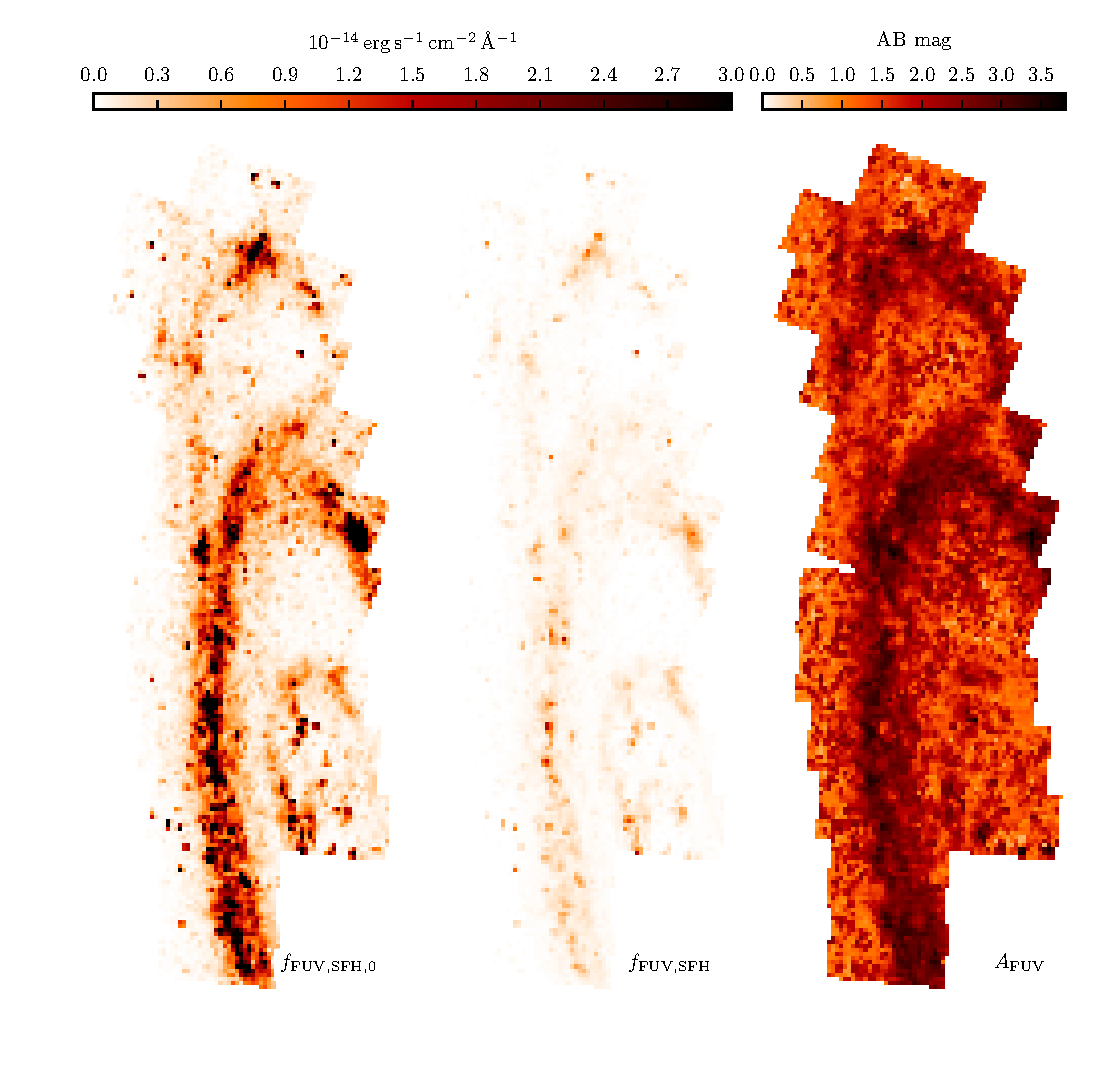
\includegraphics[width=\textwidth]{m31flux-figures/modfluxmaps_fuv.pdf}
\caption[\fuv{} flux map modeled from the \sfh{s}.]{\fuv{} flux modeled from
    the \sfh{s}. The intrinsic flux, \ffuvsfhz{}, is shown in the left panel
    and the middle panel shows the flux attenuated according to the extinction
    model, \ffuvsfh{} (also shown alongside the observed GALEX \fuv{} flux in
    Figure \ref{fig:iv}). The \fuv{} extinction, \afuv{}, derived
    from \ffuvsfhz{} and \ffuvsfh{} is shown on the right.
}
\label{fig:ii}
\end{figure*}
}


\def \figiii {
\begin{figure*}
\centering
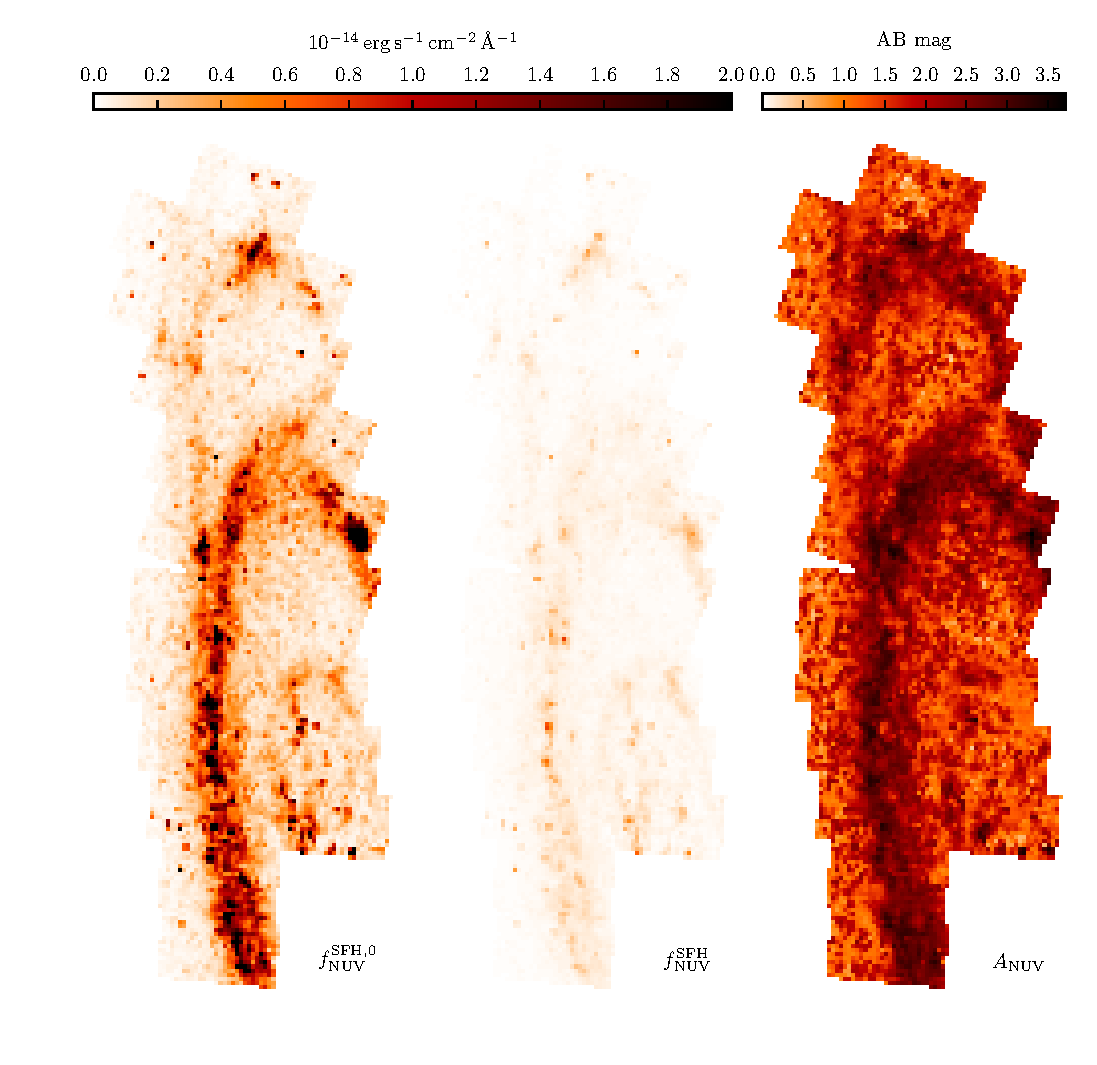
\includegraphics[width=\textwidth]{m31flux-figures/modfluxmaps_nuv.pdf}
\caption[\nuv{} flux map modeled from the \sfh{s}.]{Same as Figure
    \ref{fig:ii}, but for the \nuv{} filter.
}
\label{fig:iii}
\end{figure*}
}


\def \figiv {
\begin{figure*}
\centering
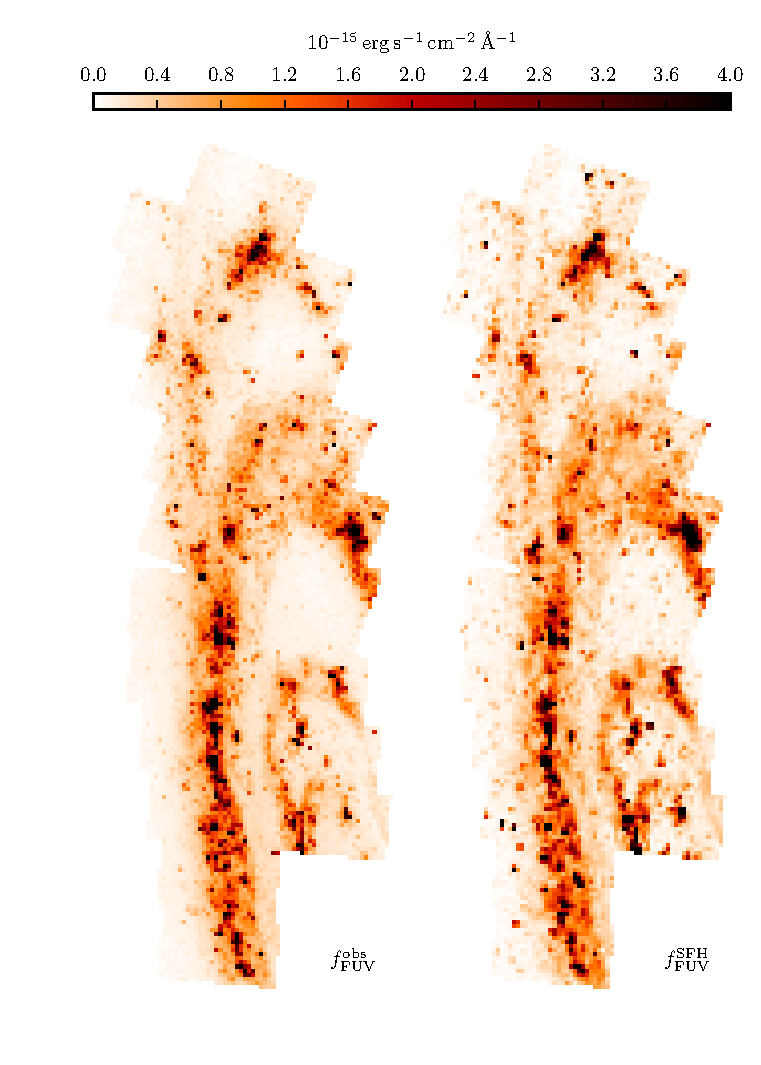
\includegraphics[scale=0.9]{m31flux-figures/fluxmaps_fuv.pdf}
\caption[Observed and synthetic attenuated \fuv{} flux maps.]{Observed \fuv{}
    flux from GALEX, \ffuvobs{} (left), and synthetic attenuated \fuv{} flux
    from the \sfh{s}, \ffuvsfh{} (right). The observed map has been clipped to
    the PHAT survey border to match the synthetic map. The synthetic fluxes
    show excellent morphological agreement with the observed fluxes.
}
\label{fig:iv}
\end{figure*}
}


\def \figv {
\begin{figure*}
\centering
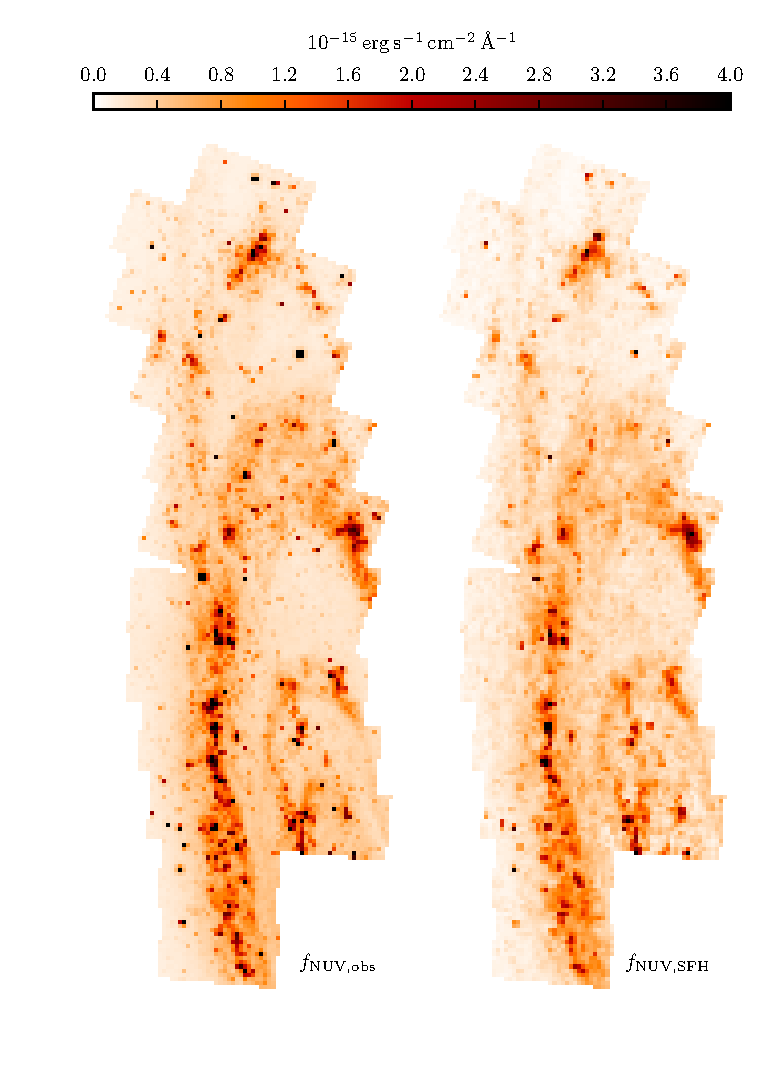
\includegraphics[scale=0.9]{m31flux-figures/fluxmaps_nuv.pdf}
\caption[Observed and synthetic attenuated \nuv{} flux maps.]{Same as Figure
    \ref{fig:iv}, but for the \nuv{} filter.
}
\label{fig:v}
\end{figure*}
}


\def \figvi {
\begin{figure*}
\centering
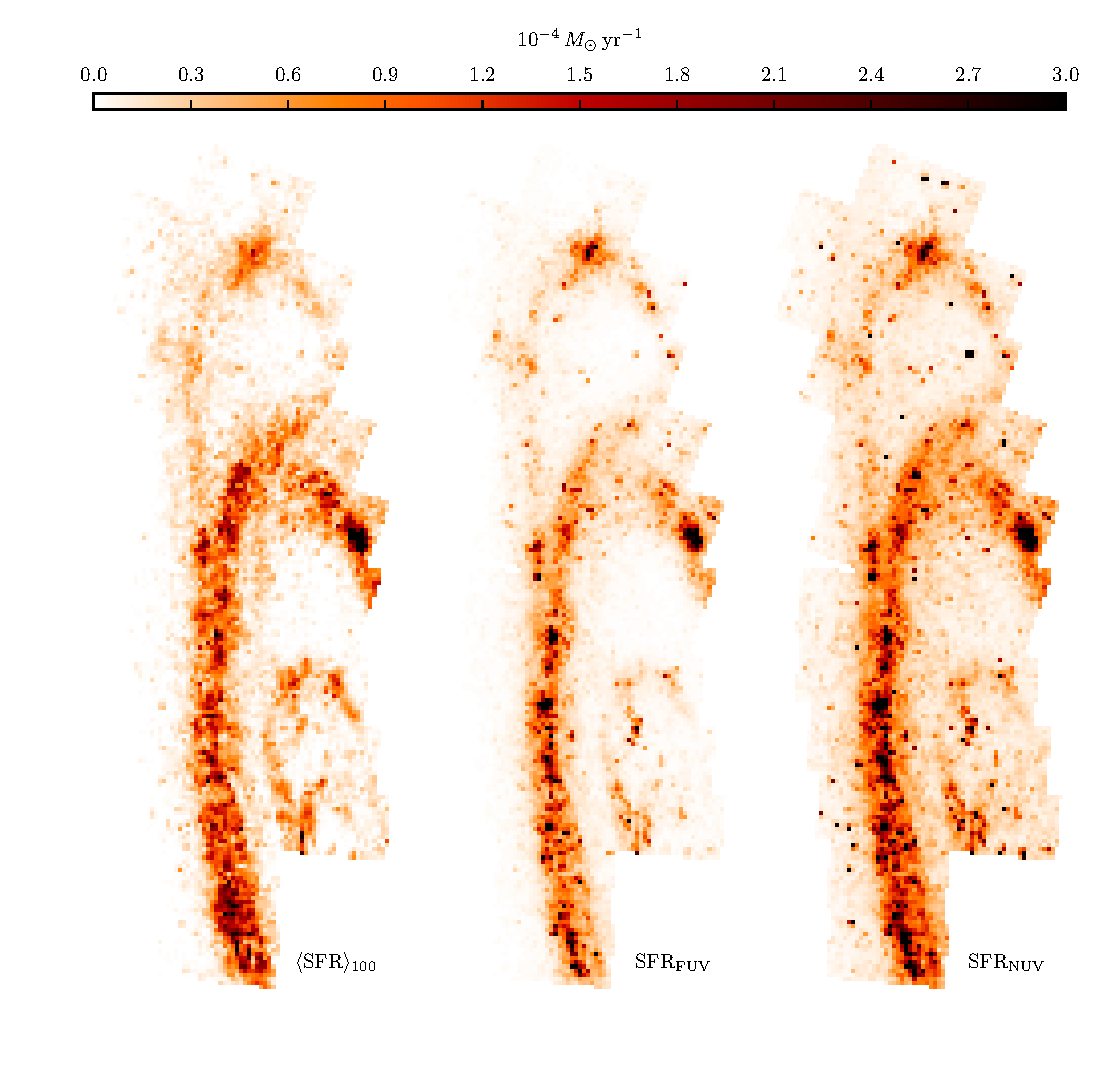
\includegraphics[width=\textwidth]{m31flux-figures/sfrmaps1.pdf}
\caption[\sfr{} maps from estimates based on observed fluxes compared with the
mean \sfr{} map from the \sfh{s}.]{\fuv{} and \nuv{} flux-based \sfr{s},
    \sfrfuv{} (middle) and \sfrnuv{} (right), compared with \sfroneh{} (left),
    the mean \sfr{} over the last $100\myr$ of the \sfh{s}. The flux-based
    \sfr{s} were derived from the observed GALEX fluxes, \ffuvobs{} and
    \fnuvobs{} (Figures \ref{fig:iv} and \ref{fig:v}),
    corrected for extinction using \afuv{} and \anuv{} (Figures
    \ref{fig:ii} and \ref{fig:iii}). The \sfr{} maps
    show good overall agreement.
}
\label{fig:vi}
\end{figure*}
}


\def \figvii {
\begin{figure*}
\centering
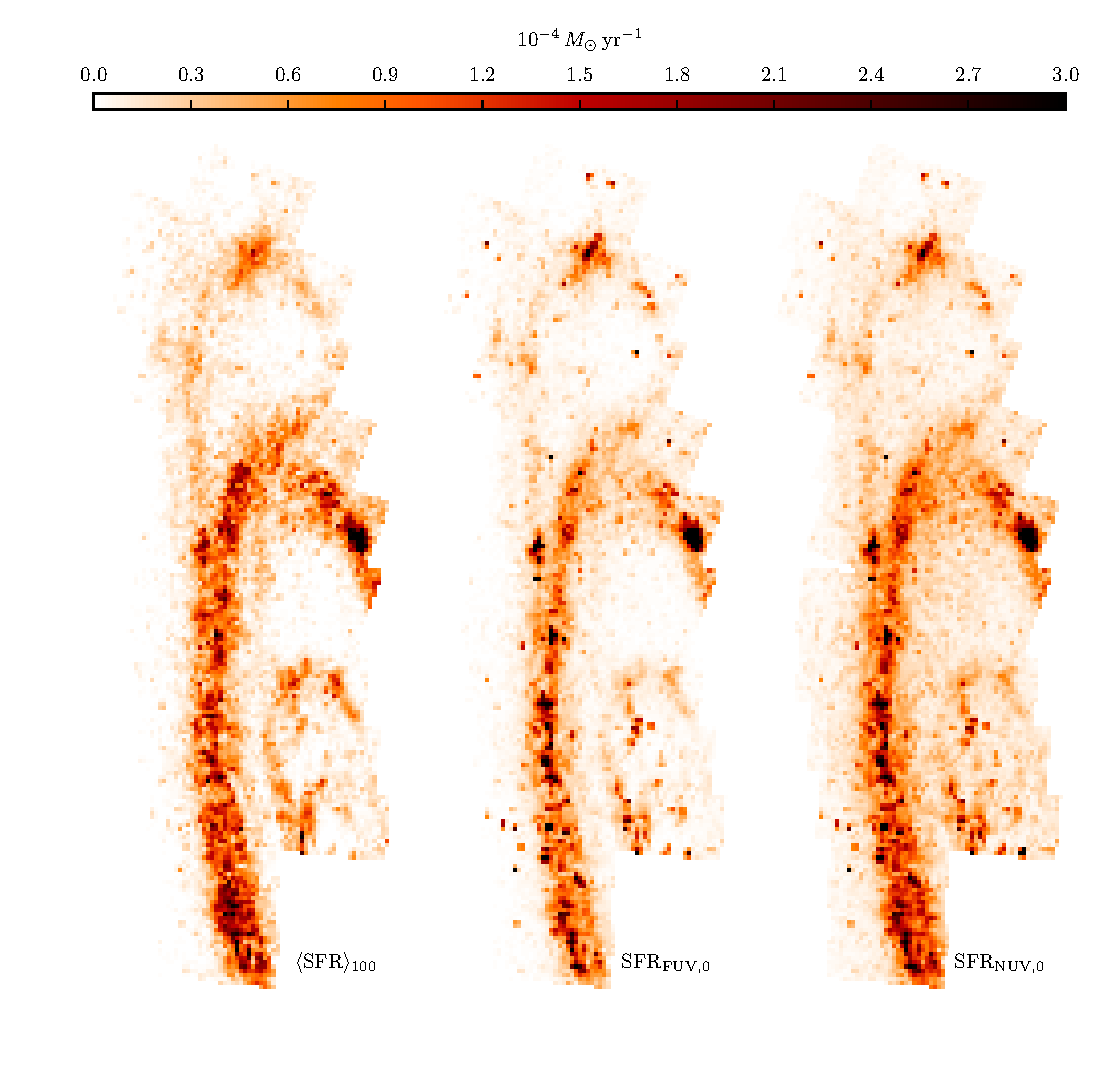
\includegraphics[width=\textwidth]{m31flux-figures/sfrmaps2.pdf}
\caption[\sfr{} maps from estimates based on synthetic intrinsic fluxes
compared with the mean \sfr{} map from the \sfh{s}.]{Same as Figure
    \ref{fig:vi}, but instead comparing \sfroneh{} with \sfrfuvz{} and
    \sfrnuvz{}, the \sfr{s} from the synthetic intrinsic (i.e., unattenuated)
    fluxes from Figures \ref{fig:ii} and \ref{fig:iii}.
    The synthetic intrinsic fluxes were derived assuming a fully populated IMF
    so there is no inconsistency with the flux calibration, which assumes the
    same. Like the \sfr{s} based on observed flux, these \sfr{s} also show good
    agreement with \sfroneh{}.
}
\label{fig:vii}
\end{figure*}
}


\def \figviii {
\begin{figure*}
\centering
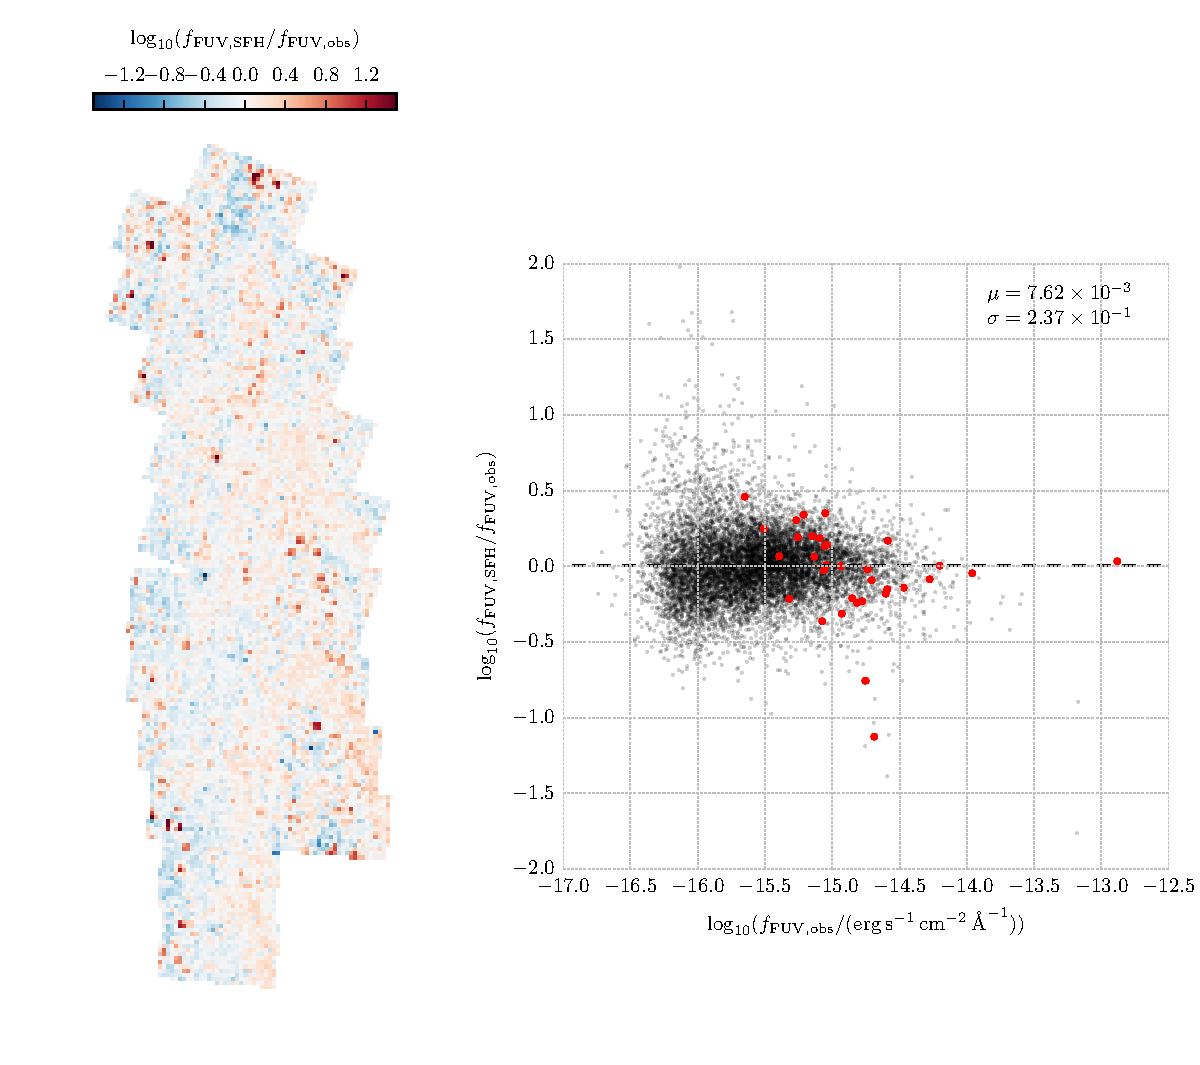
\includegraphics[width=\textwidth]{m31flux-figures/flux_fuv_sfh-vs-obs.pdf}
\caption[Ratio of the synthetic flux to the observed flux in the \fuv{}
filter.]{Ratio of the synthetic attenuated flux, \ffuvsfh{}, to the GALEX
    observed flux, \ffuvobs{}, in the \fuv{} filter. The log flux ratios in the
    scatter plot follow a normal distribution with $\mu = 7.62\times 10^{-3}$
    (horizontal dashed line) and $\sigma = 2.37\times 10^{-1}$. The median
    ratio is 1.02 with 68\% confidence limits of 0.59 and 1.76. \ffuvsfh{} and
    \ffuvobs{} are therefore consistent on average. The flux ratio variance
    increases with decreasing observed flux, suggesting that the uncertainties
    are dominated by incomplete IMF sampling. The large red circles represent
    flux ratios for the UV-bright regions from \citet{Simones:2014} and are
    consistent with the main sample. The map shows a fairly even spatial
    distribution for the flux ratios, with the most severely overestimated and
    underestimated pixels occurring primarily in the faint, off-arm areas of
    the galaxy, as shown in the scatter plot.
}
\label{fig:viii}
\end{figure*}
}


\def \figix {
\begin{figure*}
\centering
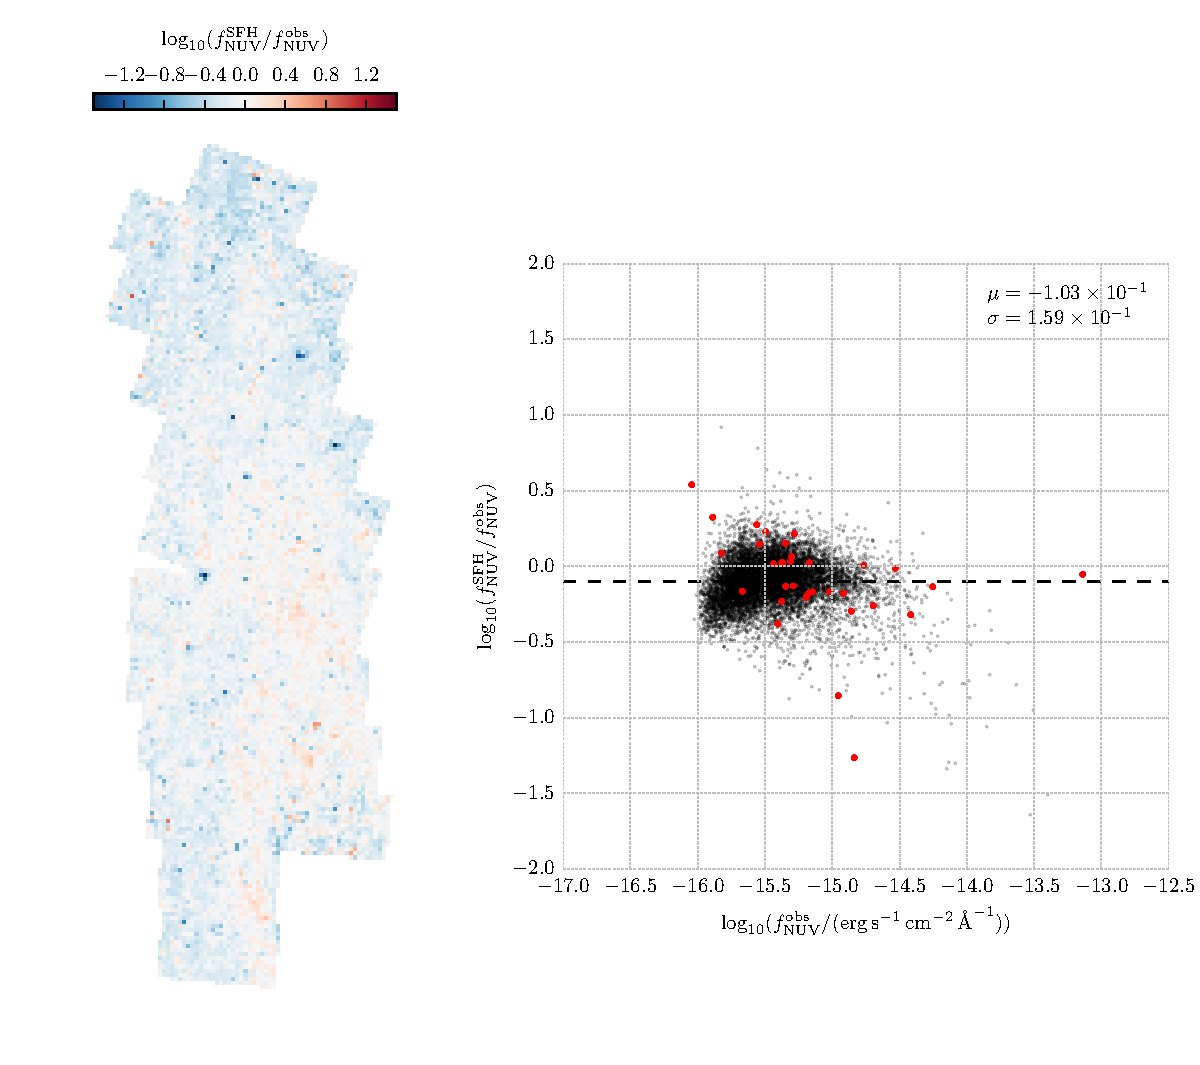
\includegraphics[width=\textwidth]{m31flux-figures/flux_nuv_sfh-vs-obs.pdf}
\caption[Ratio of the synthetic flux to the observed flux in the \nuv{}
filter.]{Same as Figure \ref{fig:viii}, but for the \nuv{} filter. In
    this case, the log-normal distribution is characterized by $\mu =
    -1.03\times 10^{-1}$ and $\sigma = 1.59\times 10^{-1}$. The median ratio is
    0.79 with 68\% confidence limits of 0.55 and 1.14. \fnuvsfh{} and
    \fnuvobs{} are therefore consistent on average. The role of IMF sampling is
    not as important for \fnuvobs{}, so the uncertainties in \fnuvsfh{} are
    somewhat smaller.
}
\label{fig:ix}
\end{figure*}
}


\def \figx {
\begin{figure*}
\centering
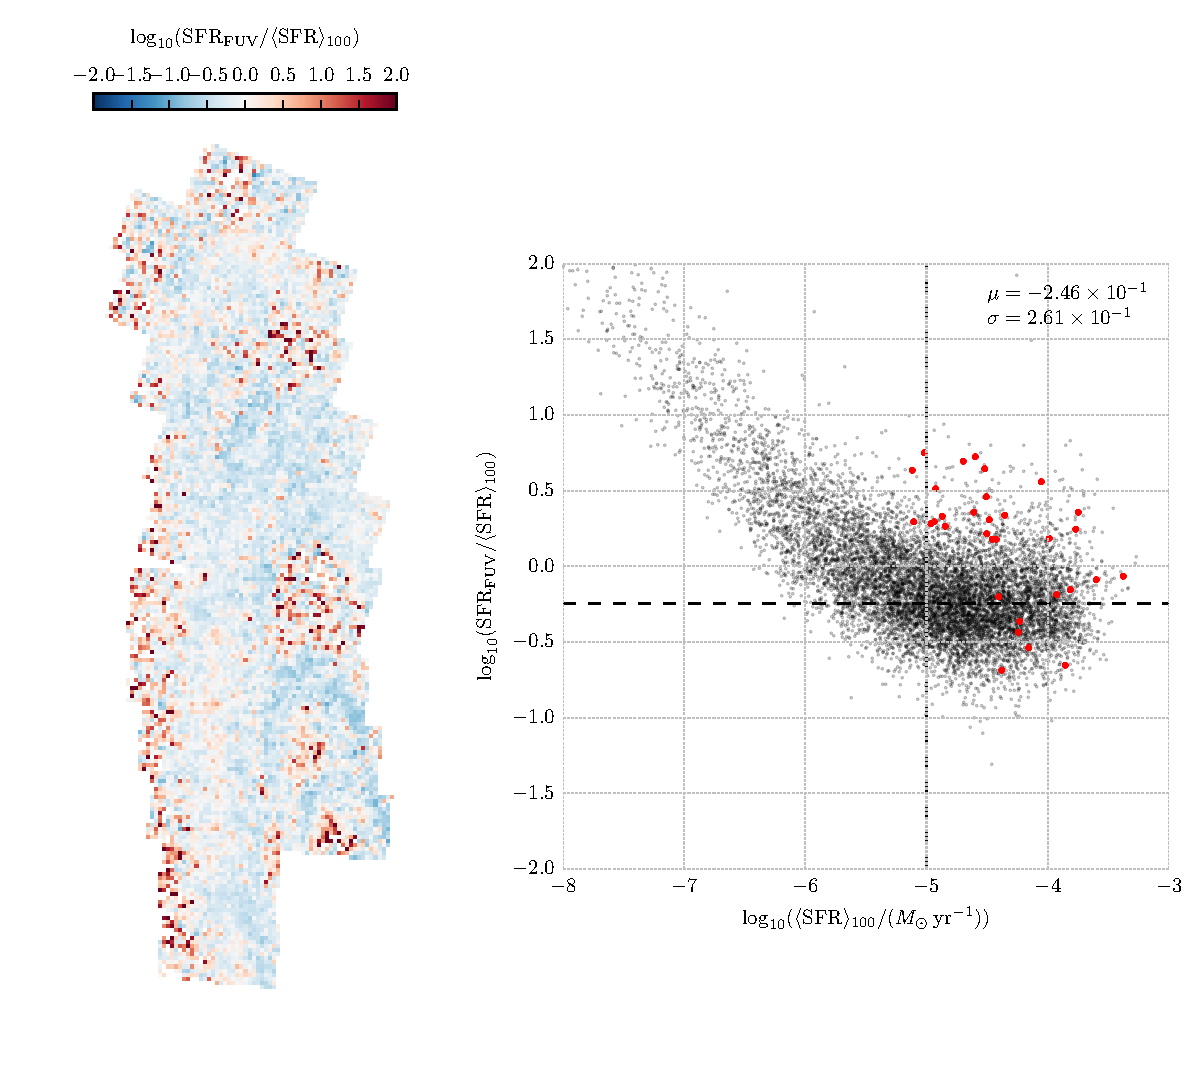
\includegraphics[width=\textwidth]{m31flux-figures/sfr_fuv-vs-mean.pdf}
\caption[Ratio of the \sfr{} based on the observed extinction-corrected \fuv{}
flux to the $100\myr$ mean \sfr{}.]{Ratio of the \sfr{} based on the observed
    extinction-corrected \fuv{} flux, \sfrfuv{}, to the $100\myr$ mean of the
    \sfh{}, \sfroneh{}. The log \sfr{} ratios show a linear tail feature with
    $-1$ slope and $-6.0$ intercept, implying that \sfrfuv{} becomes constant
    for $\sfroneh < 9.8\times 10^{-7}\msun\yr^{-1}$. We constrain our analysis
    to pixels with $\sfroneh10^{-5}\msun\yr^{-1}$ (vertical dashed line). Above
    this limit, the log \sfr{} ratios follow a normal distribution with $\mu =
    -2.46\times 10^{-1}$ (horizontal dashed line) and $\sigma = 2.61\times
    10^{-1}$. The median ratio is 0.57 with 68\% confidence limits of 0.31 and
    1.04, most likely due to incomplete IMF sampling. \sfrfuv{} and \sfroneh{}
    are therefore consistent on average. The large red circles represent \sfr{}
    ratios for the UV-bright regions from \citet{Simones:2014} and are
    consistent with the main sample. Apart from the faint, off-arm areas
    responsible for the tail feature, the map shows a fairly even spatial
    distribution for the \sfr{} ratios.
}
\label{fig:x}
\end{figure*}
}


\def \figxi {
\begin{figure*}
\centering
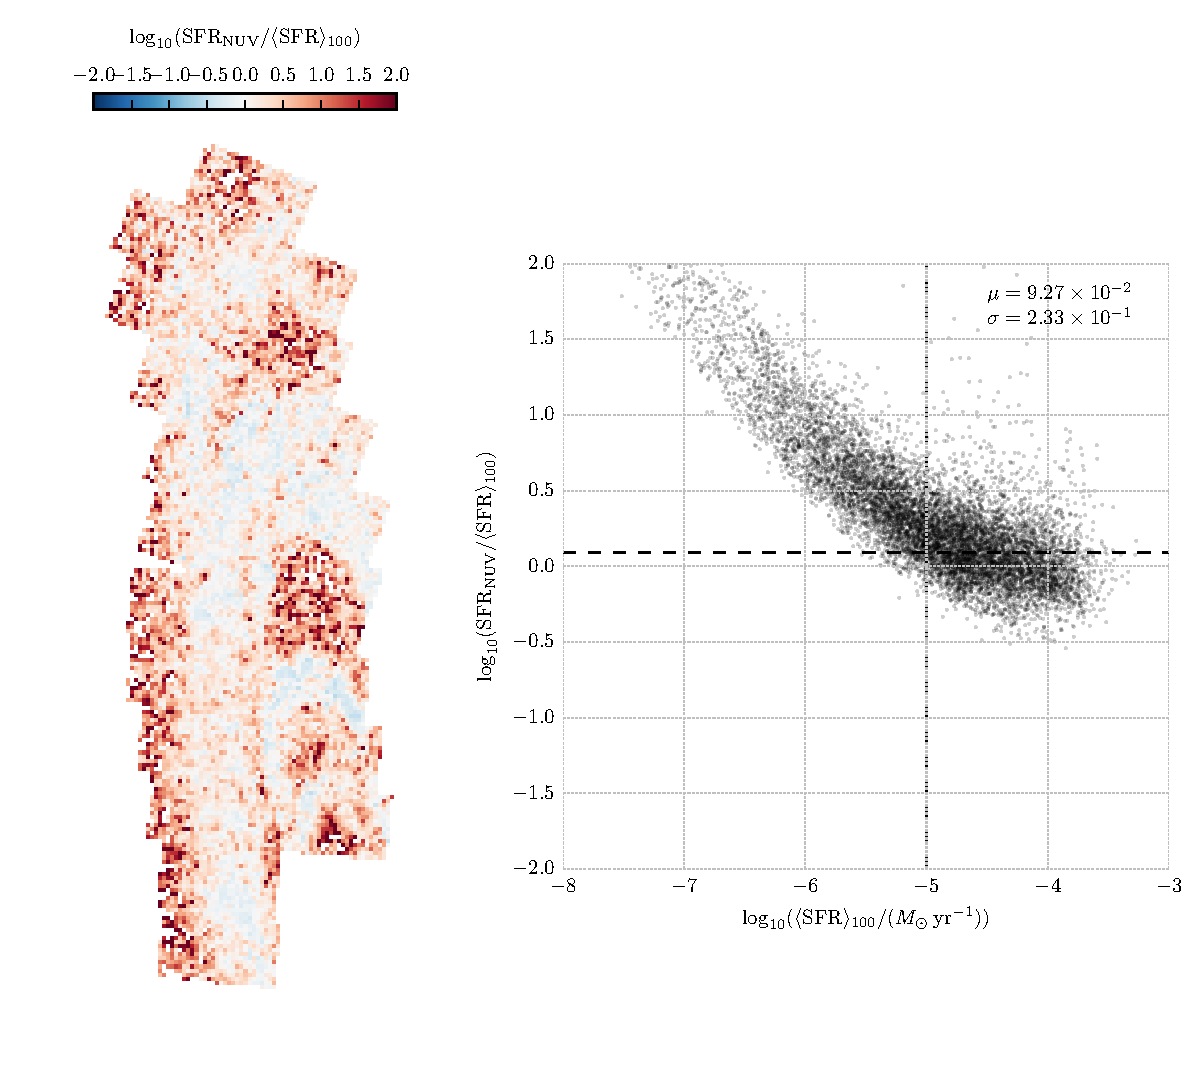
\includegraphics[width=\textwidth]{m31flux-figures/sfr_nuv-vs-mean.pdf}
\caption[Ratio of the \sfr{} based on the observed extinction-corrected \nuv{}
flux to the $100\myr$ mean \sfr{}.]{Same as Figure \ref{fig:x}, but
    for the \nuv{} filter. In this case, the linear tail has an intercept of
    $-5.4$ such that \sfrnuv{} becomes constant for $\sfroneh < 4.1\times
    10^{-6}\msun\yr^{-1}$. The log-normal distribution is characterized by $\mu
    = 9.27\times 10^{-2}$ and $\sigma = 2.33\times 10^{-1}$. The median ratio
    is 1.24 with 68\% confidence limits of 0.72 and 2.12. \sfrnuv{} and
    \sfroneh{} are therefore consistent on average.
}
\label{fig:xi}
\end{figure*}
}


\def \figxii {
\begin{figure*}
\centering
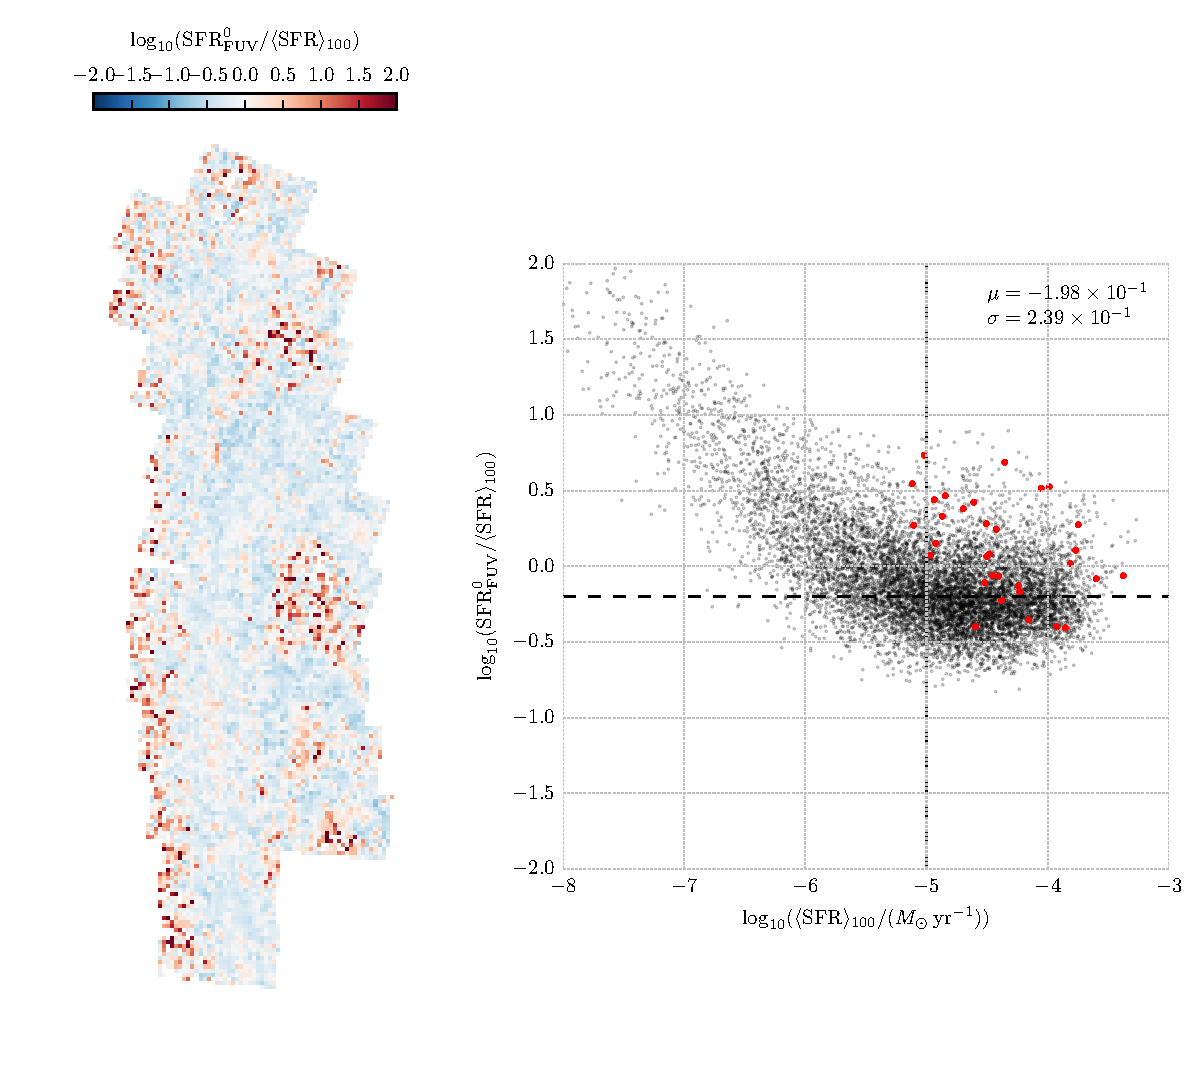
\includegraphics[width=\textwidth]{m31flux-figures/sfr_fuv0-vs-mean.pdf}
\caption[Ratio of the \sfr{} based on the synthetic intrinsic \fuv{} flux to
the $100\myr$ mean \sfr{}.]{Same as Figure \ref{fig:x}, but based on
    synthetic instrinsic flux, \sfrfuvz{}. The log-normal distribution is
    characterized by $\mu = -1.98\times 10^{-1}$ and $\sigma = 2.39\times
    10^{-1}$. The median ratio is 0.63 with 68\% confidence limits of 0.37 and
    1.10. \sfrfuvz{} and \sfroneh{} are therefore consistent on average. The
    results here are similar to Figure \ref{fig:x}, suggesting that
    \sfh{} variability does not significantly affect the \sfrfuv{}
    uncertainties.
}
\label{fig:xii}
\end{figure*}
}


\def \figxiii {
\begin{figure*}
\centering
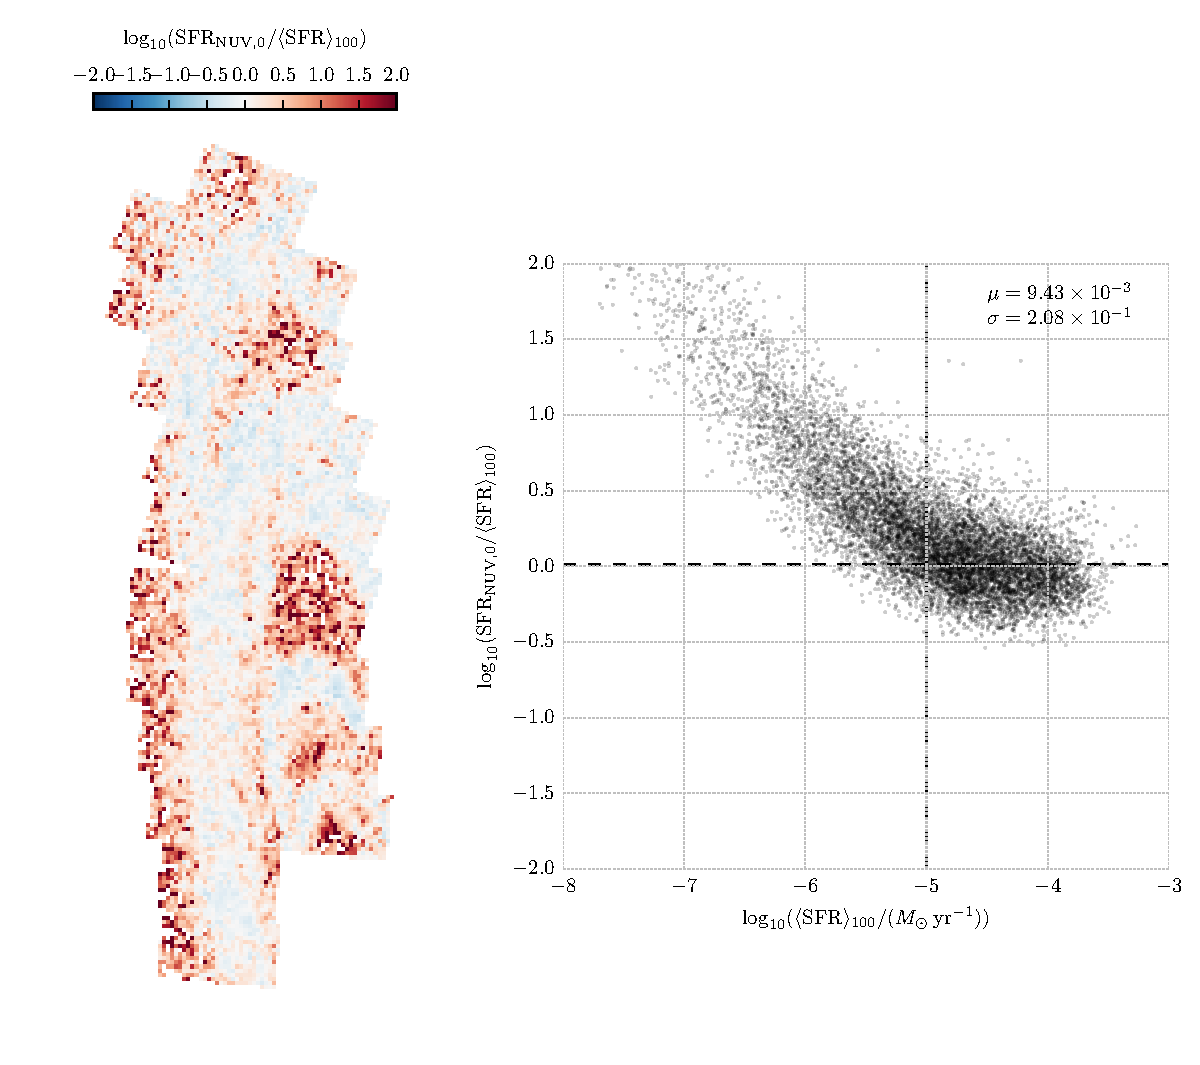
\includegraphics[width=\textwidth]{m31flux-figures/sfr_nuv0-vs-mean.pdf}
\caption[Ratio of the \sfr{} based on the synthetic intrinsic \nuv{} flux to
the $100\myr$ mean \sfr{}.]{Same as Figure \ref{fig:xi}, but based on
    synthetic instrinsic flux, \sfrnuvz{}. The log-normal distribution is
    characterized by $\mu = 9.43\times 10^{-3}$ and $\sigma = 2.08\times
    10^{-1}$. The median ratio is 1.02 with 68\% confidence limits of 0.63 and
    1.65. \sfrnuvz{} and \sfroneh{} are therefore consistent on average. The
    results here are similar to Figure \ref{fig:xi}, suggesting that
    \sfh{} variability does not significantly affect the \sfrnuv{}
    uncertainties.
}
\label{fig:xiii}
\end{figure*}
}


\def \tabi {
\begin{deluxetable}{lcc}
\tabletypesize{\footnotesize}
\tablecaption{\emph{GALEX} filter properties.\label{tab:i}}
\tablewidth{0pt}
\tablehead{
    &
    \colhead{FUV} &
    \colhead{NUV}
}
\startdata
Unit response, $U_\filter$ \\
$(\times 10^{-15}\uflambda)$\tablenotemark{a} &  1.40 &  0.206 \\
\\
AB magnitude \\
zeropoint, $Z_\filter$\tablenotemark{a} &  18.82 &  20.08 \\
\\
Effective wavelength ($\!\ang$)\tablenotemark{b} &  1538.6 &  2315.7
\enddata
\tablenotetext{a}{\url{http://galexgi.gsfc.nasa.gov/docs/galex/FAQ/counts\_background.html}}
\tablenotetext{b}{\citet{Morrissey:2007}}
\end{deluxetable}


%\begin{deluxetable}{ccc}
%\tabletypesize{\footnotesize}
%\tablecaption{\emph{GALEX} filter properties.\tablenotemark{a}\label{tab:i}}
%\tablewidth{0pt}
%\tablehead{
%    \colhead{Filter} &
%    \colhead{$U_\filter \, (\erg\ssec^{-1}\cm^{-2}\ang^{-1})$\tablenotemark{b}} &
%    \colhead{$Z_\filter \, \mathrm{(mag)}$\tablenotemark{c}}
%}
%\startdata
%FUV &  $1.40 \times 10^{-15} $ &  18.82 \\
%NUV &  $2.06 \times 10^{-16} $ &  20.08
%\enddata
%\tablenotetext{a}{\url{http://galexgi.gsfc.nasa.gov/docs/galex/FAQ/counts\_background.html}}
%\tablenotetext{b}{Unit response.}
%\tablenotetext{c}{AB magnitude zeropoint.}
%\end{deluxetable}

}


\def \tabii {
\begin{deluxetable}{cc}
\tabletypesize{\footnotesize}
\tablecaption{\emph{GALEX} observations.\label{tab:ii}}
\tablewidth{0pt}
\tablehead{
    \colhead{Filter} &
    \colhead{Tile name}
}
\startdata
FUV &  \texttt{PS\_M31\_MOS00-fd-int.fits} \\
    &  \texttt{PS\_M31\_MOS07-fd-int.fits} \\
    &  \texttt{PS\_M31\_MOS08-fd-int.fits} \\
    &  \texttt{PS\_M31\_MOS09-fd-int.fits} \\
    &  \texttt{PS\_M31\_MOS10-fd-int.fits} \\
NUV &  \texttt{PS\_M31\_MOS00-nd-int.fits} \\
    &  \texttt{PS\_M31\_MOS07-nd-int.fits} \\
    &  \texttt{PS\_M31\_MOS08-nd-int.fits} \\
    &  \texttt{PS\_M31\_MOS09-nd-int.fits} \\
    &  \texttt{PS\_M31\_MOS10-nd-int.fits}
\enddata
\end{deluxetable}

}


\def \tabiii {
\newlength{\dy}
\setlength{\dy}{2pt}

\begin{deluxetable*}{ccccccc}
\tabletypesize{\footnotesize}
\tablecaption{Results.\label{tab:iii}}
\tablewidth{0pt}
\tablehead{
    \colhead{Figure} &
    \colhead{Quantity} &
    \colhead{$\mu$\tablenotemark{a}}  &
    \colhead{$\sigma$\tablenotemark{a}} &
    \colhead{Median\tablenotemark{b}}  &
    \colhead{68\% C.L.\tablenotemark{c}} &
    \colhead{Unc.\tablenotemark{d}}
}
\startdata
\ref{fig:viii} &  $\ffuvsfh/\ffuvobs$ &   $7.62\times 10^{-3}$ &  $2.37\times 10^{-1}$ &  1.02 &  0.59, 1.76 &  $-0.43$, $+0.74$ \\[\dy]
\ref{fig:ix}   &  $\fnuvsfh/\fnuvobs$ &  $-1.03\times 10^{-1}$ &  $1.59\times 10^{-1}$ &  0.79 &  0.55, 1.14 &  $-0.24$, $+0.35$ \\[\dy]
\tablenotemark{*}\ref{fig:x}    &  $\sfrfuv/\sfroneh$  &  $-2.46\times 10^{-1}$ &  $2.61\times 10^{-1}$ &  0.57 &  0.31, 1.04 &  $-0.26$, $+0.47$ \\[\dy]
\tablenotemark{*}\ref{fig:xi}   &  $\sfrnuv/\sfroneh$  &   $9.27\times 10^{-2}$ &  $2.33\times 10^{-1}$ &  1.24 &  0.72, 2.12 &  $-0.52$, $+0.88$ \\[\dy]
\tablenotemark{*}\ref{fig:xii}  &  $\sfrfuvz/\sfroneh$ &  $-1.98\times 10^{-1}$ &  $2.39\times 10^{-1}$ &  0.63 &  0.37, 1.10 &  $-0.27$, $+0.47$ \\[\dy]
\tablenotemark{*}\ref{fig:xiii} &  $\sfrnuvz/\sfroneh$ &   $9.43\times 10^{-3}$ &  $2.08\times 10^{-1}$ &  1.02 &  0.63, 1.65 &  $-0.39$, $+0.63$
\enddata
\tablenotetext{a}{$\mu$ and $\sigma$ represent the location and scale parameters
    of the quantity's log-normal distrubution.}
\tablenotetext{b}{Calculated from the location parameter as $10^{\mu}$.}
\tablenotetext{c}{Lower and upper 68\% confidence limits, $10^{\mu\pm\sigma}$.}
\tablenotetext{d}{Lower and upper uncertainties as the difference between the
    median and the 68\% confidence limits.}
\tablenotetext{*}{Statistics apply only to pixels with $\sfroneh \ge
    10^{-5}\msun\yr^{-1}$.}
\end{deluxetable*}

}






\begin{document}

\title{The Panchromatic Hubble Andromeda Treasury. \textsc{XXX}. Synthetic
    ultraviolet flux maps of M31 from resolved optical
    photometry.\footnotemark[*]
}

\footnotetext[*]{Based on observations made with the NASA/ESA \emph{Hubble Space
    Telescope}, obtained from the Data Archive at the Space Telescope Science
    Institute, which is operated by the Association of Universities for Research
    in Astronomy, Inc., under NASA contract NAS 5-26555.
}

\author{Jacob E. Simones\altaffilmark{1},
    Alexia R. Lewis\altaffilmark{2},
    Benjamin D. Johnson\altaffilmark{4},
    Julianne J. Dalcanton\altaffilmark{2},
    Andrew E. Dolphin\altaffilmark{3},
    Evan D. Skillman\altaffilmark{1},
    Daniel R. Weisz\altaffilmark{4,5},
    Benjamin F. Williams\altaffilmark{2}
}

\altaffiltext{1}{Minnesota Institute for Astrophysics, University of Minnesota,
    116 Church Street SE, Minneapolis, MN 55455, USA; jsimones@astro.umn.edu;
    skillman@astro.umn.edu
}
\altaffiltext{2}{Department of Astronomy, Box 351580, University of Washington,
    Seattle, WA 98195, USA; jd@astro.washington.edu; ben@astro.washington.edu
}
\altaffiltext{3}{Raytheon, 1151 E. Hermans Road, Tucson, AZ 85756, USA;
    adolphin@raytheon.com
}
\altaffiltext{4}{Department of Astronomy, University of California at Santa
    Cruz, 1156 High Street, Santa Cruz, CA 95064, USA; drw@ucsc.edu,
    bjohnso6@ucsc.edu
}
\altaffiltext{5}{Hubble Fellow}

\shortauthors{Simones et al.}





\begin{abstract}

Starting from star formation histories based on color magnitude diagrams, we
have used stellar population synthesis to create maps of synthetic far- and
near-ultraviolet (\fuv{} and \nuv{}) flux at sub-kpc resolution for the
northeast quadrant of M31. The synthetic maps reproduced all of the main
morphological features found in corresponding maps of observed \fuv{} and
\nuv{} flux, including rings and large star-forming complexes. Comparing the
flux maps pixel-by-pixel, we found the median synthetic-to-observed flux ratios
to be $1.02 \;+\!0.74/\!-\!0.43$ in \fuv{} and $0.79 \;+\!0.35/\!-\!0.24$ in
\nuv{}. The synthetic fluxes were therefore consistent overall with the
observed fluxes in both filters. We used the observed fluxes and standard flux
calibrations to derive star formation rate (\sfr{}) maps, which we compared
with a map of the mean \sfr{s} over the last $100\myr$ of the star formation
histories (\sfh{s}). We determined a lower limit of $\sfr \sim
10^{-5}\msun\yr^{-1}$ below which the commonly assumed linear relationship
between UV flux and \sfr{} appears to break down. Above this limit, we found
the median ratios of the flux-based \sfr{s} to the mean \sfr{s} to be $0.57
\;+\!0.47/\!-\!0.26$ in \fuv{} and $1.24 \;+\!0.88/\!-\!0.52$ in \nuv{}. Both
the \fuv{} and \nuv{} flux-based \sfr{s} were therefore consistent overall with
the mean \sfr{s} derived from the \sfh{s}. Integrating over the entire mean
\sfr{} map, we found a global \sfr{} of $0.3\msun\yr^{-1}$. The corresponding
measurements from the flux-based \sfr{} maps were factors of 0.74 (\fuv{}) and
1.45 (\nuv{}) of the global mean \sfr{} value. It is not yet understood why the
\sfr{} ratios in the global case are larger than the median pixel-wise ratios.
The primary source of uncertainty in both the synthetic flux maps and the
flux-based \sfr{} maps was most likely incomplete IMF sampling due to the small
pixel areas. With the exception of the faintest areas of the galaxy, we did not
identify any trends for flux or \sfr{} with environment.

%TODO
%   Dan: I’m very particular about the abstract, since most readers only read
%   this, and will only read the paper if the abstract is very compelling. I
%   think the abstract in the draft was missing a few things (e.g., a reference
%   to PHAT) and was maybe not quite pitched to as broad an audience as I think
%   will be interested in the paper.
%
%   I’ve tried re-crafting your abstract:
%
%   We explore the reliability of widely used ultra-violet (UV) star formation
%   rate (SFR) indictors on sub-kpc scales using optical \emph{HST} imaging of
%   resolved stars in M31 taken as part of the Panchromatic Hubble Andromeda
%   Treasury program (PHAT). Using star formation histories (SFHs) derived from
%   optical color-magnitude diagram (CMD) analysis and population synthesis
%   code, we construct synthetic \emph{GALEX} maps with a physical revolution of
%   ~0.04 kpc^2 and compare them with actual \emph{GALEX} FUV and NUV
%   observations of M31. The synthetic UV maps reproduce all of the main
%   morphological features in the \emph{GALEX} imaging, including rings and
%   large star-forming complexes. We compare synthetic and observed FUV and NUV
%   flux maps and find flux ratios of order unity, indicating excellent overall
%   agreement, despite only using optical data in the construction of the
%   synthetic UV maps.  Maps of the mean SFRs over the last 100 Myr show that
%   the FUV SFR indicator is reliable for SFRs > 10^5 Msun/yr, and SFRs > xx
%   Msun/yr for the NUV, when averaged over 200 Myr.  We find variations in the
%   SFH can introduce modest scatter above these SFR limits.  Below 10^-5
%   Msun/yr, the UV contributions of older populations (300 Myr or is it even
%   older???) cannot be ignored and may form the dominant source of diffuse UV
%   emission in galaxies (e.g., the inter-arm regions in M31). (XXX add
%   something about the IMF if you think it’s an important effect)  Integrated
%   over the entire PHAT area, we find a mean SFR over the past 100 Myr of ~0.3
%   Msun/yr, compared to 0.22 Msun/yr from the observed FUV flux and 0.43
%   Msun/yr from the observed NUV flux. While these results are in good
%   qualitative agreement, the modest differences may be due to global
%   fluctuations in M31’s recent SFH, uncertainties in the treatment of dust
%   attenuation, or the less understood UV properties of older stellar
%   populations.
%
%
%   Abstract: If the global ratios are different than the median of the pixel
%   ratios, the distribution must be asymmetric.  Figs 12 and 13 certainly
%   suggest this is the case.  Perhaps make a cumulative histogram to show just
%   how asymmetric the distribution is, and make a comparison without the tail.

\end{abstract}

\keywords{galaxies: evolution --
    galaxies: individual (M31) --
    galaxies: photometry --
    galaxies: star formation --
    galaxies: stellar content
}





\section{Introduction}

%TODO
%   Alexia: A little more motivation here would help, especially getting into
%   the second paragraph. Why are we modeling the flux? What's in the literature
%   about flux modeling? How has it been done before? What needs to be improved?

M31 is a well-studied, large spiral galaxy and has been observed at a variety of
wavelengths, e.g., in the ultraviolet (UV) by the \emph{Galaxy Evolution
Explorer} \citep[\emph{GALEX};][]{Morrissey:2007}, in the optical, including
H$\alpha$, for the Local Group Galaxies Survey \citep{Massey:2006}, and in the
infrared by the \emph{Spitzer Space Telescope} \citep{Gordon:2006}. The wealth
of high-quality data available for M31 provides a valuable opportunity to model
various observations and test our current understanding of stellar astrophysics.
%TODO
%   Alexia: Disjointed? Maybe add more connecting and explanatory material here.
In particular, the initial mass function (IMF), models of stellar evolution and
stellar spectra, and extinction curves are all required to model the integrated
light from galaxies.

%TODO
%   BenW: Put all of the examples of wavelengths in to one large parenthetical
%   statement, or leave it out of parentheses and break it up into a couple of
%   sentences.

%TODO
%   Dan: Para 1: Broad intro to how in order to understand galaxy evolution, we
%   rely on interpreting the integrated light of distant galaxies across cosmic
%   time. There are a bunch of assumptions built into how this works (e.g., SFH,
%   IMF, etc) which we either fix or parameterize in order to accommodate the
%   available observations (e.g., we assume tau model SFHs because they are
%   simple and seem reasonable). We also want to connect gas to stars to
%   understand SF (e.g., Leroy, Biegel et al.) and often rely on integrated SF
%   tracers (e.g., Halpha, FUV, etc).

%TODO
%   BenW: After the first paragraph, a more comprehensive review of the subject
%   should be added.  A few more paragraphs putting your work in context and
%   referencing any highly cited related work would go a long way (a few
%   examples of integrated light galaxy survey results that rely heavily on pop
%   synthesis models, Ben Johnson's work, etc.).  Then you can move into the
%   current paragraph 2 with a stronger motivation.

A critical ingredient for modeling the flux from a galaxy is a detailed
knowledge of its star formation history (\sfh{}). Deriving \sfh{s} by
color-magnitude diagram (CMD) analysis is a reliable method that can be used
whenever photometry of resolved stars is available. An extensive optical
photometric catalog for M31 has been compiled by the Panchromatic Hubble
Andromeda Treasury \citep[PHAT;][]{Dalcanton:2012,Williams:2014}, and
\citet{Lewis:2015} have used these data to derive the spatially resolved \sfh{}
of the northeast quadrant. With sub-kpc resolution, this \sfh{} dataset is the
ideal input for stellar population synthesis codes that model total flux given a
population's star formation rate (\sfr{}) and metallicity evolution. The result
is a set of spatially resolved maps of synthetic broadband flux in M31 which can
be compared with observations.

%TODO
%   Dan: Para 2: But many of these assumptions are untested on different spatial
%   scales and in different types of environments.  For examples, several
%   studies have shown SFR tracers to be less reliable in low luminosity/mass
%   systems (e.g., Lee et al. 2009, Meurer et al. 2009) which may be attributed
%   to IMF sampling issues (e.g., da Silva et al. 2012, 2014) or variability in
%   SFHs (e.g., Weisz et al. 2013a). However, tests of these results have been
%   limited to low-metallicity dwarf galaxies, which are not representative of
%   environments in which most stars in the universe form.

\figi
%TODO
%   Alexia: For this and all other figures: more description of the figures in
%   the text.

The \citet{Lewis:2015} \sfh{s} can also be used to create temporally averaged
\sfr{} maps. Because the \sfh{s} were derived from the resolved stars without
any prior assumptions about the \sfh{s}, such maps provide a standard against
which flux-based \sfr{} estimates \citep[e.g., using any of the calibrations
from][]{Kennicutt:2012} can be tested. Using integrated flux to estimate \sfr{s}
for distant galaxies, where resolved stars are not available, is a common
technique in extragalactic astronomy. Previous studies have investigated how
flux-based \sfr{} estimators hold up against resolved-star \sfh{s} in sub-kpc
UV-bright regions \citep{Simones:2014} and in low-metallicity dwarf galaxies
\citep{Johnson:2013,McQuinn:2015}. The \sfh{s} of \citet{Lewis:2015} based on
data from PHAT make it possible to broaden this type of analysis to include a
wide variety of environments in a large local group spiral galaxy.

%TODO
%   Dan: “without any prior assumptions” -> not quite true.  MATCH assumes some
%   things, e.g., SF is constant over a time bin, the linear sum of SSPs makes
%   up a galaxy.  These are many fewer assumptions than typical SFH work (which
%   assume a parametric SFH model, for example), but it is not assumption free.

%TODO
%   Dan: Para 3: Fortunately, with observations from PHAT we can now test the
%   validity of these assumptions using resolved stars.  Describe PHAT briefly —
%   don’t assume everyone just knows what it is.  Describe that we can
%   accurately measure SFHs on small spatial scaled using CMD analysis. Describe
%   how we can then use these secure SFHs to make predictions of fluxes in other
%   filters to test SFR indicators, among other things.

In this study, we have used the PHAT CMD-based \sfh{s} and stellar population
synthesis to create maps of synthetic UV flux at sub-kpc resolution for the
northeast quadrant of M31. We then compared the synthetic flux maps with
observations from \emph{GALEX}. We have focused only on \emph{GALEX} \fuv{} and
\nuv{} (far and near UV), though this work can be extended to other wavelength
regimes. In \S \ref{syntheticfluxmaps}, we describe the \sfh{} dataset and the
production of the synthetic flux maps. \S \ref{observations} describes the
process of producing observed flux maps from \emph{GALEX} \fuv{} and \nuv{}
images. The creation of \sfr{} maps both from the \sfh{s} and the observed
fluxes using common flux-\sfr{} calibrations are described in \S
\ref{sfrestimates}. In \S \ref{discussion}, we compare the synthetic maps with
the observations and compare mean \sfr{} maps with \sfr{s} estimated from
observed flux. We conclude in \S \ref{conclusion}.

%TODO
%   Dan: Para 4-6: Mention that we did preliminary work in Simones et al. 2014.
%   Here we build on that work by doing the following….last bit: this paper is
%   organized as follows:





\section{Synthetic UV flux maps}\label{syntheticfluxmaps}



\subsection{The spatially resolved star formation history of M31}\label{syntheticfluxmaps:sfhs}

The PHAT survey \citep{Dalcanton:2012,Williams:2014} measured multiband
photometry for over 117 million resolved stars in M31 using the \emph{Hubble
Space Telescope} (\emph{HST}). The PHAT survey area is shown in Figure
\ref{fig:i}. \citet{Lewis:2015} used photometry in the two optical bands
(\acsb{} and \acsi{}, observed with the Advanced Camera for Surveys, ACS,
instrument) to derive spatially resolved \sfh{s} for the northeast quadrant of
M31, excluding the crowded bulge area. To summarize their work, each brick
(using PHAT terminology; see Figure \ref{fig:i}) in the PHAT survey (except
bricks 1 and 3) was divided into 450 regions on a uniform $15 \times 30$ grid,
with each region $\sim 24\aarcsec \times 27\aarcsec$ in size. The $\acsb,\acsi$
CMD of each region was then fit using the CMD modeling code MATCH
\citep{Dolphin:2002} to determine the most likely \sfh{} under the following
assumptions:

\begin{enumerate}
\item The \citet{Kroupa:2001} IMF.
\item The Padova isochrones \citep{Marigo:2008} with updated asymptotic giant
    branch tracks \citep{Girardi:2010}.
\item A binary fraction of 0.35 with a uniform mass ratio.
\item A distance modulus of 24.47 \citep{McConnachie:2005}.
\item Age resolutions of $0.1\dex$ for $6.60 \le \logten(\mathrm{age}) \le 9.90$
    and $0.25\dex$ for $9.90 < \logten(\mathrm{age}) \le 10.15$.
\item A metallicity resolution of $0.1\dex$ over the range $-2.3 \le \met \le
    0.1$, constrained to increase monotonically over time.
\item A two-parameter extinction model consisting of a total foreground
    component, \avf{}, and an additional differential component following a
    uniform distribution from 0 to a maximum value, \dav{}. The \avf{} and
    \dav{} parameters were optimized for each region \citep[see
    also][]{Simones:2014}.
\end{enumerate}

In addition, the portion of each CMD with $\acsb - \acsi > 1.25$ and $\acsb >
21$ (red giant branch and red clump stars) was excluded from the fit. This was
done to ensure that the optimized extinction parameters corresponded only to the
dust associated with the young, UV-producing stars on the main sequence.



\subsection{Broadband UV flux modeling}\label{syntheticfluxmaps:fluxmod}

We used the \sfh{s} (\S \ref{syntheticfluxmaps:sfhs}) to model broadband UV
fluxes, allowing us to create synthetic UV flux maps for the PHAT survey area.
Past studies have used CMD-based \sfh{s} to model fluxes, including
\citet{Gogarten:2009} for UV-bright regions in the outer disk of M81,
\citet{Johnson:2013} for dwarf galaxies in the Local Volume, and more recently
\citet{Simones:2014} for a small sample of UV-bright regions in M31. Our work
builds directly on the analysis of \citet{Simones:2014} by extending our
coverage to the entire PHAT survey area to include a wide variety of
environments. We focused on modeling fluxes in the \emph{GALEX} \fuv{} and
\nuv{} filters only. However, because we begin by modeling spectral energy
distributions (SEDs), the process we describe below can be generalized to model
fluxes in any set of filters assuming the range of ages covered by the SFHs is
sufficient.
%TODO
%   Ben: Move the "Past studies..." part (most of this paragraph) to the intro?

The flux in a given region was modeled using a technique based on that described
in \citet{Johnson:2013}. We began with a set of simple stellar population (SSP)
models generated using the Flexible Stellar Population Synthesis (FSPS) code
\citep{Conroy:2009, Conroy:2010}. For consistency with \citet{Lewis:2015}, we
ran FSPS assuming the \citet{Kroupa:2001} IMF and the Padova isochrones
\citep{Marigo:2008} with updated asymptotic giant branch tracks
\citep{Girardi:2010}. We also chose the BaSeL 3.1 semi-empirical stellar SED
library \citep{Westera:2002}. The SSPs were aged from $\log(\mathrm{age})=5.500$
to 10.175 in steps of $0.025\dex$. We set the SSP metallicities independently
for each region using the mean metallicity over the last $100\myr$ of the \sfh{}
(the $100\myr$ timescale corresponds to the lifetime of UV emission). If the
\sfr{} was consistently zero over the last $100\myr$, then we instead set the
metallicity to the most recent metallicity where $\sfr > 0$.

We applied the SSP models to a region's \sfh{} to model its integrated SED. We
first processed the \sfh{} by rescaling the youngest age bin to include all ages
up to the present (the Padova isochrones are only available for
$\logten(\mathrm{age}) \ge 6.60$), and increasing the age resolution of the full
\sfh{} to 20 samples per age bin. The subsampled \sfh{} was then interpolated to
the series of ages in the set of SSP models. The SED of each SSP was weighted by
the mass of its corresponding age bin from the \sfh{}, and the individual SSP
SEDs were finally summed to derive the integrated intrinsic (i.e., unattenuated)
model SED.

\tabi

\figii
%TODO
%   For this and all other maps:
%   - Add a scale bar indicating, e.g., 1 kpc
%   - Use a gray background? Does it look better to have the maps set apart from
%     the white of the page?

%TODO
%   For this and Figure 3:
%   - Change A_FUV to A_FUV^SFH
%   - A_FUV stretch is too dark.

\figiii

We derived an attenuated SED for the region using the same two-component
extinction model used by MATCH to fit the CMD together with the region's
best-fit \avf{} and \dav{} parameters \citep{Lewis:2015}. To do this, we divided
the intrinsic SED into 30 identical component SEDs (larger numbers of components
did not significantly improve the accuracy of our results). Each component was
attenuated according to the \citet{Cardelli:1989} extinction curve with a
uniform random $A_\mathrm{V}$ drawn between \avf{} and $\avf + \dav$. The
\citet{Cardelli:1989} extinction curve predicts the amount of extinction
relative to that in the V band, $A_\mathrm{V}$, as a function of wavelength and
is based on the average extinction in the Galaxy with a total-to-selective
extinction ratio of $\rv = 3.1$. Previous studies have shown that this
extinction curve is applicable to M31 as a whole in both the UV
\citep{Bianchi:1996} and the optical \citep{Barmby:2000} regimes. Finally, the
attenuated SED components were summed to obtain the region's integrated
attenuated model SED.

The intrinsic and the attenuated model SEDs were weighted by the response curves
for the \emph{GALEX} \fuv{} and \nuv{} filters to obtain absolute synthetic
\fuv{} and \nuv{} magnitudes in the AB system. The absolute magnitudes were
converted into apparent magnitudes for the region by assuming a distance modulus
of 24.47 \citep{McConnachie:2005}.

Using a subscript (indicated here by \filter{}) to refer to either \fuv{} or
\nuv{}, the conversion between absolute magnitude, $m_\filter$, and flux,
$f_\filter$, in filter \filter{} is given by,
%
\begin{equation}
m_\filter = -2.5 \log_{10}\left(\frac{f_\filter}{U_\filter}\right)
    + Z_\filter \; ,
\label{eq:magtoflux}
\end{equation}
%
where the \emph{GALEX} unit responses, $U_\filter$, and zeropoints, $Z_\filter$,
are given in Table \ref{tab:i}. We used the apparent magnitudes and Equation
\ref{eq:magtoflux} to derive the intrinsic and the attenuated broadband UV
fluxes for the region, denoted by \fxsfhz{} and \fxsfh{}, respectively.

After modeling the intrinsic and attenuated fluxes for all of the regions in a
brick, we assembled the flux values (for a given filter) into a $15 \times 30$
array to form an image mapping the synthetic flux across the brick. The brick
map was independently tied to a world coordinate system using a 2D least-squares
optimization to find the best-fit CD matrix \citep{Calabretta:2002} for a
gnomonic tangent plane projection using the known RA and DEC coordinates of the
brick grid vertices measured by \citet{Lewis:2015}. We repeated this process for
all of the bricks, resulting in a set of 21 brick maps. We then reprojected and
added the brick maps using
Montage\footnote{\url{http://montage.ipac.caltech.edu/}} to create full maps,
or mosaics, of synthetic \fuv{} and \nuv{} flux for the PHAT survey area.

All of the mosaic maps are registered to a grid defined by a template header
that was automatically chosen by Montage as the best fit to the collection of
input brick maps. The mosaic grid has a pixel scale of $23.75\aarcsec$, which
is comparable to the sizes of the regions from the original brick grids defined
in \citet{Lewis:2015}. Assuming a distance modulus of 24.47
\citep{McConnachie:2005}, a disk inclination of $78\ddeg$ \citep{Tully:1994},
and a major axis position angle of $35\ddeg$ \citep{deVaucouleurs:1995}, the
pixel scale is deprojected to a linear size of $dx = 440\pc$ and $dy = 100\pc$
approximately along the minor and major axes of M31, respectively. The
synthetic flux maps therefore have a resolution that is firmly in the sub-kpc
regime.

The final synthetic flux maps, \fxsfhz{} and \fxsfh{}, are shown in Figures
\ref{fig:ii} (\fuv{}) and \ref{fig:iii}
(\nuv{}).\footnote{\label{github}The synthetic and the observed flux maps, as
well as the $100\myr$ mean \sfr{} map, are available at
\url{https://github.com/jesaerys/m31flux}.}

We used the synthetic flux maps to derive maps of \ax{}, the total extinctions
in the \fuv{} and \nuv{} bands. The intrinsic and attenuated flux maps were
converted into AB magnitudes, \xsfhz{} and \xsfh{}, using Equation
\ref{eq:magtoflux}. The extinction maps were then calculated as the difference
between the attenuated and the intrinsic magnitudes, $\ax = \xsfh - \xsfhz$. We
show the synthetic extinction maps with their corresponding synthetic flux maps
in Figures \ref{fig:ii} and \ref{fig:iii}.
%TODO
%   Alexia: describe the figures

A pixel weight map representing the coverage of the available PHAT data was
also produced during the mosaicking process. Mosaic pixels fully within the
PHAT survey border (excluding bricks 1 and 2 near the bulge) have a weight of
1, pixels fully outside the border have a weight of 0, and all other pixels
have weights between 0 and 1 depending on the fraction of the pixel area within
the survey border. Throughout this study we used the weight map to mask out all
pixels not fully within the survey border so that our comparisons with
observations are done on a full-pixel basis.





\section{\emph{GALEX} observations}\label{observations}

\tabii

\figiv
%TODO
%   Alexia: describe the figures

\figv

We constructed maps of observed \emph{GALEX} \fuv{} and \nuv{} flux, \fxobs{},
to match the synthetic flux maps described in \S
\ref{syntheticfluxmaps:fluxmod}. We started with the intensity maps of five
tiles in the \emph{GALEX} Deep Imaging Survey \citep[DIS;][]{Martin:2005}
covering the PHAT survey area (see Table \ref{tab:ii}). The tiles were
converted from count rate units, $\mathrm{cps}$, into flux according to,
%
\begin{equation}
f_\filter = U_\filter \left(\frac{\mathrm{cps}_\filter}{
    \mathrm{counts} \ssec^{-1} \,\mathrm{pixel}^{-1}}\right) \; ,
\label{eq:cpstoflux}
\end{equation}
%
where $U_\filter$ is given in Table \ref{tab:i}. We then used Montage to
reproject the flux tiles to the same template header as the synthetic flux
mosaics (see \S \ref{syntheticfluxmaps}), match the background levels of the
tiles, and add the tiles together to create the final mosaic.

A small amount of background UV flux was present in the \fuv{} and \nuv{}
mosaics, primarily due to scattering of UV photons from hot foreground stars in
the Galaxy. We measured the mean background flux in a rectangular aperture in an
off-galaxy area relatively devoid of stars in the reprojected,
background-matched tile \texttt{PS\_M31\_MOS07}. The resulting \fuv{} and \nuv{}
background levels were slightly underestimated and overestimated, respectively,
causing a significant downturn/upturn in the distribution of the $\fxsfh/\fxobs$
ratios for pixels with \fxobs{} comparable to the background. To correct for
this, we adjusted the background levels such that the median
$\logten(\fxsfh/\fxobs)$ value for all pixels with $\fxobs <
10^{-15.5}\uflambda$ (the approximate median of \fxobs{}) matched that for all
of the brighter pixels. The adjusted background values were $5.22 \times
10^{-19}$ and $3.47 \times 10^{-19}\uflambda\aarcsec^{-2}$ ($2.9 \times
10^{-16}$ and $2.0 \times 10^{-16}\uflambda$ per mosaic pixel) in \fuv{} and
\nuv{}, respectively. We subtracted these values from the \fuv{} and \nuv{}
mosaics to obtain the final observed UV flux maps for the PHAT survey area,
\fxobs{}, shown in Figures \ref{fig:iv} (\fuv{}) and \ref{fig:v} (\nuv{}).

We emphasize that pixels with values comparable to the background ($\fxobs \sim
10^{-15.5}\uflambda$) or fainter in Figures \ref{fig:iv} and \ref{fig:v} are
highly sensitive to the background subtraction method. This effect is
particularly important for the distribution of the $\fxsfh/\fxobs$ ratios among
the faint areas in the UV maps (\S \ref{discussion:modflux}). For the brighter
pixels, the background subtraction method makes little difference.





\section{\sfr{} estimates}\label{sfrestimates}

\figvi
%TODO
%   Mention in the caption the part from the Discussion about point sources
%   found in one map but not the other.

\figvii

A common method for estimating the \sfr{} of a target is to measure the
integrated flux in one or more filters and then calculate the \sfr{} using one
of the flux-to-\sfr{} calibrations available in the literature, e.g., (for UV
flux) those discussed by \citet{Kennicutt:1998}, \citet{Salim:2007},
\citet{Hao:2011}, \citet{Murphy:2011}, and \citet{Leroy:2012}; see also the
review by \citet{Kennicutt:2012}. We used this method to derive \sfr{} maps for
the PHAT survey area, which we later compared with similar maps derived from the
\sfh{s} (\S \ref{syntheticfluxmaps:sfhs}), extending the work of
\citet{Simones:2014} to a much larger sample that is more diverse in terms of UV
brightness and star formation activity.

To calculate flux-based \sfr{s}, we converted the \fxobs{} maps into AB
magnitudes, \xobs{}, (Equation \ref{eq:magtoflux}) which we corrected for
extinction by subtracting the synthetic \ax{} maps (\S
\ref{syntheticfluxmaps:fluxmod}). The extinction-corrected maps were converted
back into (specific) fluxes ($\!\uflambda$), then into total fluxes ($\erg
\ssec^{-1} \cm^{-2}$) by multiplying by the effective filter wavelengths in
Table \ref{tab:i}. The total fluxes were converted into luminosities, \lx{}
($\erg \ssec^{-1}$), assuming a distance modulus of 24.47
\citep{McConnachie:2005}. Finally, we applied the calibrations from
\citet{Kennicutt:1998} with updates by \citet{Hao:2011} and \citet{Murphy:2011}
\citep[see the review by][]{Kennicutt:2012} to obtain the \fuv{} and \nuv{}
flux-based \sfr{} estimates, \sfrx{}, respectively:
%
\begin{equation} \left(\frac{\sfrfuv}{\msun\yr^{-1}}\right) =
10^{-43.35}\,\left(\frac{\lfuv}{\erg\ssec^{-1}}\right) \label{eq:fuvcal}
\end{equation}
%
\begin{equation} \left(\frac{\sfrnuv}{\msun\yr^{-1}}\right) =
10^{-43.17}\,\left(\frac{\lnuv}{\erg\ssec^{-1}}\right) \label{eq:nuvcal}
\end{equation}
%
These calibrations are based on stellar population synthesis using Starburst99
\citep{Leitherer:1999} and assume a constant \sfr{} over the last $100\myr$, the
\citet{Kroupa:2001} IMF, a fully populated range of masses from 0.1 to
$100\msun$, and solar metallicity \citep{Hao:2011}.

The most robust flux calibrations are the those that rely on more than one part
of the electromagnetic spectrum. An example of a hybrid estimator is the
combination of \emph{GALEX} \fuv{} and \emph{Spitzer} $24\,\mu\mathrm{m}$
fluxes, which simultaneously accounts for the direct starlight from newly formed
massive stars and the absorbed starlight processed and reradiated by dust
\citep[e.g.,][]{Leroy:2012}. However, we have limited our study to observations
by \emph{GALEX}, so we will only consider the simpler monochromatic \fuv{} and
\nuv{} calibrations in Equations \ref{eq:fuvcal} and \ref{eq:nuvcal}. We show
the final \sfrx{} maps in Figure \ref{fig:vi}.

To help determine the importance of SFH variability on the SFRs calculated from
Equations \ref{eq:fuvcal} and \ref{eq:nuvcal} (see \S \ref{discussion:sfrs}), we
created another pair of flux-based \sfr{} maps derived as before, except we
started with the intrinsic synthetic fluxes \fxsfhz{} described in \S
\ref{syntheticfluxmaps:fluxmod}. Because the fluxes were intrinsic, it was not
necessary to apply an extinction correction before converting the fluxes into
\sfr{s}. The maps for the intrinsic flux-based \sfr{} estimates, \sfrxz{}, are
shown in Figure \ref{fig:vii}.

\tabiii

We also created a map for the mean \sfr{} over the past $100\myr$ of the
\sfh{s}, \sfroneh{}, which we show alongside the flux-based \sfr{} maps in
Figure \ref{fig:vi}. The $100\myr$ limit represents the nominal timescale of UV
emission and matches the timescale used by \citet{Hao:2011} to derive the \fuv{}
and the \nuv{} flux calibrations.





\section{Discussion}\label{discussion}
%TODO
%   Be sure to emphasize that we're using *optical* data to make predictions
%   about UV.

%TODO
%   Dan: Cite previous work (in the introduction as well?) on SFR indicators at
%   low SFR: Lee et al. 2009, Meurer et al. 2009, Boselli et al. 2009, da Silva
%   2012, 2014, Cervino et al. 2012.


\subsection{Modeled flux}\label{discussion:modflux}

Figures \ref{fig:iv} and \ref{fig:v} show remarkable overall qualitative
agreement between the synthetic attenuated fluxes \fxsfh{} (derived from optical
CMDs) and the observed \emph{GALEX} fluxes \fxobs{}. In particular, all of the
main features brighter than $\sim 10^{-15}\uflambda$ in the observed maps are
reproduced in the synthetic maps. This includes the main rings at $\sim 5$, 10,
and $15\kpc$ from the center of M31, and the large star-forming complexes found
in PHAT bricks 15 and 21. However, in detail we find distinct differences
between the \fxsfh{} and \fxobs{}. Possible sources for these differences are
discussed below.

The \fxobs{} maps show several point sources which are not present in the
\fxsfh{} maps. These are most likely foreground stars that are lost in the
synthetic maps because the fluxes were not derived for individual stars, but
from SFHs that correspond to the \emph{distributions} of stars in the CMDs.
Likewise, there are some apparent point sources in the \fxsfh{} maps that are
not in the \fxobs{} maps. We attribute these to photometric artifacts (e.g.,
diffraction spikes) remaining in the PHAT photometry despite applied quality
puts \citep{Dalcanton:2012}. The presence of photometric artifacts in a region
increases the stellar mass measured in the region's SFH, thereby increasing the
synthetic flux. Although foreground stars and photometric artifacts ruin the
comparison between \fxsfh{} and \fxobs{}, such contamination only affects a
small minority of the pixels in the maps.

We compare the synthetic and observed fluxes more quantitatively in Figures
\ref{fig:viii} (\fuv{}) and \ref{fig:ix} (\nuv{}), which map the ratio of
\fxsfh{} to \fxobs{} over the PHAT survey area. The Figures also show the flux
ratios as a function of \fxobs{}. We find that the log flux ratios follow normal
distributions with mean $\mu = 7.62\times 10^{-3}$ and standard deviation
$\sigma = 2.37\times 10^{-1}$ for \fuv{}, and $\mu = -1.03\times 10^{-1}$ and
$\sigma = 1.59\times 10^{-1}$ for \nuv{}. In linear terms, the median flux
ratios are 1.02 in \fuv{} and 0.79 in \nuv{}, with 68\% confidence limits of
0.59 and 1.76 (\fuv{}) and 0.55 and 1.14 (\nuv{}). These results are summarized
in Table \ref{tab:iii}. Note that in both filters, the median ratio is within
the confidence interval of 1, indicating that \fxsfh{} is overall consistent
with \fxobs{}.

\figviii
%TODO
%   For this and similar figures:
%   - Add histograms along both axes of the scatter plot to show the 1-d
%     distributions.
%   - Black dashed line is hard to see. Either make it a standout color or
%     lighten the scatter points.
%   - Tick labels are a bit crowded. E.g., maybe just use -17, -16, -15, etc. on
%     the x axis.

\figix

The overall agreement between \fxsfh{} and \fxobs{} shows that our modeling
procedure is generally robust and justifies the several key assumptions used to
derive \fxsfh{} from the optical CMDs. Specifically, we assumed an IMF, models
describing stellar spectra and evolution, and an extinction model as well as an
extinction curve. These form the foundation for much research in astronomy and
encompass our current best understanding of stellar astrophysics and star
formation. It is therefore reassuring that we can use all of this knowledge to
derive \sfh{s}, synthesize SEDs, and successfully recreate detailed maps of a
galaxy, all from photometry in just two optical bands.

The Poisson uncertainties in \fxobs{} are relatively small. Assuming an average
exposure time of $7\times 10^3\ssec$ in the \fuv{} channel for the five DIS
images in our study, the uncertainties are only a few percent at $\ffuvobs \sim
10^{-16}\uflambda$ and a few tenths of a percent at $\ffuvobs \sim
10^{-14}\uflambda$. The corresponding \nuv{} uncertainties for an average
exposure time of $6\times 10^4\ssec$ in the \nuv{} channel are about one tenth
of those in the \fuv{}. However, Figures \ref{fig:viii} and \ref{fig:ix} show
variances that are much larger than the Poisson uncertainties allow. These
variances are therefore due almost exclusively to systematic effects in the
modeling process, which we discuss below.

The primary systematic effect at play is most likely incomplete sampling of the
IMF \citep{Elmegreen:1999, Bastian:2010, Fumagalli:2011, daSilva:2012,
daSilva:2014}. This explanation is supported by the observation that the
variance in the flux ratios increases with decreasing pixel brightness,
especially in the \fuv{} filter. Also, the \fxsfh{} maps show somewhat more
uneven, noisy backgrounds, i.e., faint pixels in the off-arm areas of M31,
compared with the \fxobs{} maps. The faint pixels are associated with low star
formation (SF) activity and, because all pixels are the same size, have fewer
stars than the brighter pixels covering the arms and main star-forming regions.
This leads to a violation of the full-IMF assumption used by FSPS and other
stellar population synthesis codes.

Any sample of a given total stellar mass can have a higher (or lower) proportion
of high-mass stars than expected for a fully populated IMF. There will therefore
be more (or less) high-energy photons than stellar population synthesis models
suggest, and the synthetic UV flux will be underestimated (or overestimated). In
other words, when a stellar population is small, the same total mass could be
produced by a variety of mass functions (samplings of the IMF), where each mass
function has its own unique luminosity. This sampling effect results in a
variance in the flux ratios that increases with decreasing surface brightness.
We observe that this trend is more pronounced in \fuv{}, as mentioned above, due
to the increased sensitivity of \ffuvobs{} to slight variations in the number of
high-mass stars relative to \fnuvobs{}.

Although IMF sampling more severely affects the fainter pixels, the sub-kpc
resolution of our flux maps results in small pixel areas such that IMF sampling
is likely the dominant source of the variance for all of the flux ratios.
Accounting for projection effects in the disk, the physical area of each pixel
is $4.4\times 10^4\pc^2$ (\S \ref{syntheticfluxmaps:fluxmod}). This is
approximately equal to the average area of the UV-bright regions considered by
\citet{Simones:2014}, who showed that the uncertainties in fluxes modeled for
UV-bright regions decreases with increasing area. They also showed that
combining several small regions into a larger $\sim\kpc$-sized region greatly
improved the agreement between the synthetic and observed fluxes. Taken
together, these results show that the best way to comply with the full-IMF
assumption and reduce the uncertainties in \fxsfh{} is to make the mosaic pixel
size larger, thereby increasing the number of stars sampled. Naturally, reducing
uncertainties this way comes at the cost of decreased spatial resolution in the
flux maps. Exploring simultaneously the effects of both surface brightness
\emph{and} pixel area on this fundamental, stochastic variance is a topic for
future study.

As discussed previously, a small subset of our data are contaminated by
foreground stars and photometric artifacts. We find that these sources of
contamination drive many of the highest and lowest ratios in Figures
\ref{fig:viii} and \ref{fig:ix}. Milky Way foreground stars can emit ultraviolet
fluxes comparable to the massive main sequence stars in M31. Excluding such
stars from the CMDs, due to, e.g., photometric quality cuts or the CMD exclusion
area, results in SFHs that (correctly) represent the stars that actually belong
to M31. This mismatch causes the observed flux to be significantly higher than
the synthetic flux, and thus leads to very low flux ratios. While many of the
highest flux ratios are consistent with discrete IMF sampling in low-flux
regions, some of the high ratios are explained by the misidentification of
photometric artifacts as massive stars in the CMDs. These lingering artifacts
contribute false mass to resulting SFHs and increase the synthetic fluxes,
dramatically increasing the flux ratios for the faintest regions.

%TODO
%   Dan: IMF sampling effects are not symmetric: there is a slight preference
%   for forming fewer high-mass stars than a full IMF over forming more
%   high-mass stars. (See Figure 3 of da Silva et al. 2014:
%   http://arxiv.org/abs/1403.4605.) This should result in some kind of
%   asymmetrical distribution such that higher ratios are more common. We might
%   be seeing hints of this in the FUV ratios.
%
%   Me: The background subtraction has a large influence on this distribution,
%   however, (\S \ref{observations}) so it's difficult to make definitive
%   claims.
%
%   Make a note somewhere in here that to really determine the importance of IMF
%   sampling on the ratio distribution, we would have to compare with
%   expectations based on some kind of simulation where we draw low-mass regions
%   from an IMF. This exercise is beyond the scope of the paper.

We have added the flux ratios for the sample of UV-bright regions in
\citet{Simones:2014} to Figures \ref{fig:viii} and \ref{fig:ix} (red circles).
Although the UV-bright regions vary in size and come from one small part of M31,
their flux ratios appear to agree with the overall distribution for the rest of
the galaxy. Also, other than the increased variance in the faint areas, we find
no obvious trends in the mean or variance of the flux ratios with respect to
environment or distance from the bulge. Therefore, we conclude that the flux
modeling procedure may be successfully applied to any population in environments
similar to M31. From the 68\% confidence limits in the flux ratio distributions,
we estimate the uncertainties in synthesizing fluxes for sub-kpc regions to be
$+\!0.74/\!-\!0.43$ and $+\!0.35/\!-\!0.24$ times the observed flux in \fuv{}
and \nuv{}, respectively (Table \ref{tab:iii}). These uncertainties are driven
mostly by incomplete sampling of the IMF and are consistent with
\citet{Simones:2014}, who found uncertainties of $+\!0.95/\!-\!0.47$ for the
synthetic \fuv{} fluxes of the UV-bright regions.
%TODO
%   BenW: Report a flux range in which these uncertainties apply.

%TODO
%   BenW: The lack of a trend in the ratios with UV brightness also suggests
%   that the IMF itself is not varying with environment. This should definitely
%   be mentioned.



\subsection{\sfr{} estimates from UV flux}\label{discussion:sfrs}
%TODO
%   Alexia: Ensure that the logic in this section flows and is easy to
%   understand.

\figx

\figxi

As with the synthetic and observed fluxes, the flux-based \sfr{} maps in Figures
\ref{fig:vi} and \ref{fig:vii} show good overall morphological agreement with
the CMD-based \sfroneh{} map. We compare the \sfr{s} more closely in Figures
\ref{fig:x} and \ref{fig:xi}, where we map the ratio of \sfrx{} to \sfroneh{}
and plot the \sfr{} ratio as a function of \sfroneh{}. A major feature in both
figures is the marked contrast in the ratios between the high \sfr{} areas and
the low \sfr{} areas. The areas with low \sfroneh{}, corresponding to the faint
areas in Figures \ref{fig:iv} and \ref{fig:v}, host nearly all of the very
highest \sfr{} ratios in the entire survey area and none of the low or moderate
ratios. The pixels in these areas make up the downward sloping tails seen at low
\sfroneh{} in the scatter plots in Figures \ref{fig:x} and \ref{fig:xi}.

The low-\sfr{} tails are distinctly linear, with slopes of $-1$ and intercepts
of $-6.0$ and $-5.4$ for the \fuv{} and \nuv{} \sfr{} ratios, respectively. In
log space, a straight line with $-1$ slope indicates that \sfrx{} becomes
constant with a value equal to $10^{-6.0} = 9.8\times 10^{-7}\msun\yr^{-1}$ for
\fuv{} and $10^{-5.4} = 4.1\times 10^{-6}\msun\yr^{-1}$ for \nuv{}. Because
\sfrx{} is directly proportional to \fxobs{}, these \sfr{} constants suggest
that there must be a constant baseline flux present in the galaxy that becomes
more apparent as \sfroneh{} decreases to very small values. Thus, the linear
relationship between flux and \sfr{} assumed by the flux calibrations in
Equations \ref{eq:fuvcal} and \ref{eq:nuvcal} appear to break down completely
below \sfroneh{} approximately one to a $\mathrm{few} \times
10^{-6}\msun\yr^{-1}$.

Using the flux calibrations in reverse, we find that the above \sfr{} constants
translate into $\ffuvobs \sim 2\times 10^{-16}\uflambda$ and $\fnuvobs \sim
8\times 10^{-16}\uflambda$ (or $-15.7$ and $-15.1$ in log flux, respectively).
Figures  \ref{fig:vi}, \ref{fig:vii}, \ref{fig:viii}, and \ref{fig:ix} show that
these flux and \sfr{} limits make the \fuv{} and \nuv{} flux-to-\sfr{}
calibrations unreliable for approximately half of the pixels in the survey area.
This demonstrates the importance of warnings in the literature
\citep[e.g.,][]{Murphy:2011,Kennicutt:2012,Leroy:2012} that flux calibrations
are problematic on sub-kpc scales. We therefore limit our analysis of the \sfr{}
ratios in Figures \ref{fig:x} and \ref{fig:xi} to pixels with \sfroneh{} greater
than a conservative threshold of $10^{-5}\msun\yr^{-1}$.

%TODO
%   BenW: How do the values where the linear relationship breaks down compare to
%   the \emph{GALEX} noise level in the data you are using?
%
%   Me: FUV and NUV background is 2.9e-16 and 2.0e-16 flux per pixel, so the
%   "breakdown" occurs in the noise.

%TODO - major
%   There needs to be some discussion about old populations here.
%
%   - There is an "old" (> at least 100 Myr) component of stars more-or-less
%     evenly spread throughout the galaxy that emit a faint UV "haze".
%   - This haze is typically of no concern because most of the time we're
%     interested in areas with recent or ongoing SF.
%   - However, in areas with very little or no recent SF, the haze constitutes a
%     significant proportion of the total flux and SFR_UV (calculated from the
%     total flux) approaches a constant "baseline" level determined by the haze.
%   - In these same areas, <SFR>_100 tends to zero because the 100 Myr limit
%     excludes the old, haze-emitting stars from the average.
%   - Therefore, we have ~log(constant/x) vs log(x), so the SFR ratio gets
%     systematically larger with decreasing <SFR>_100.
%
%   So, I think my statement that the calibrations are "completely unreliable"
%   below the haze level is not entirely fair. Rather, it might be better to say
%   that the calibrations become **misleading** because they are based on a
%   theoretical population with continuous SF over the last 100 Myr, yet SFR_UV
%   in these quiescent areas is definitely not from any recent SF. The
%   theoretical population is not a good model in these cases.
%
%   I think it might be important to emphasize that SFR_UV *is* the SFR that the
%   theoretical population would have if it produced the observed flux. It *is
%   not* the SFR of the actual population over the last 100 Myr, as measured by
%   <SFR>_100.
%
%   Dan:
%       Old populations are problematic for UV in regions of low-flux.  It’s not
%       quite as simple as extending populations models to older age though,
%       since we actually don’t understand the UV properties of this populations
%       (e.g., post-AGB stars, extreme-HB stars) very well.  But, that’s not
%       important for the paper.  Statements like SFR recipes are unreliable in
%       regions of low UV flux are good.
%
%   Ben:
%       The only thing is that even extending the timescale beyond 100 Myr might
%       not totally resolve the issue, since there would still be the assumption
%       of constant SF over that timescale when going from f^SFH to SFR^0, which
%       is clearly not the case, plus what Dan says about uncertain flux
%       modeling of older populations.  And as you say it would ruin the
%       comparisons.
%
%       Agree also about including the emphasis about what SFR_UV actually
%       means.
%
%   Scattering of UV light into and out of the regions probably also has a role
%   here, but studying this would require some kind of radiative transfer
%   analysis which is outside the scope of this project.

Considering only pixels with $\sfroneh \ge 10^{-5}\msun\yr^{-1}$, we treat the
\sfr{} ratios as having log-normal distributions with $\mu = -2.46\times
10^{-1}$ and $\sigma = 2.61\times 10^{-1}$ for \fuv{}, and $\mu = 9.27\times
10^{-2}$ and $\sigma = 2.33\times 10^{-1}$ for \nuv{} (Table \ref{tab:iii}). The
median ratios are 0.57 (\fuv{}) and 1.24 (\nuv{}), with 68\% confidence limits
of 0.31 and 1.04 (\fuv{}) and 0.72 and 2.12 (\nuv{}), indicating that \sfrx{} is
consistent with \sfroneh{} overall. However, given the small uncertainties for
the observed fluxes (\S \ref{syntheticfluxmaps:fluxmod}) the large variances of
the \sfr{} ratios suggest that significant systematic effects are involved in
the flux-to-\sfr{} conversion process. We discuss these effects, including
metallicity and IMF sampling, below.

One of the assumptions made by the flux calibrations in Equations
\ref{eq:fuvcal} and \ref{eq:nuvcal} is that the input flux is produced by a
stellar population with solar metallicity. The mean metallicity of the brick
grid regions (\S \ref{syntheticfluxmaps:fluxmod}) is $\met = -0.06$ with a
standard deviation of 0.09, so the mosaic pixels are consistent with solar
metallicity on average. From \citet{Simones:2014}, overestimating \met{} by
$0.1\dex$ causes the \sfr{} to be overestimated by $0.015\dex$. Therefore, the
variation in the metallicities contributes only $0.01\dex$ to the variation in
the log \sfr{} ratios, making metallicity unimportant for the overall \sfr{}
ratio distribution.

Like the modeled fluxes in \S \ref{discussion:modflux}, the flux calibrations
also assume a fully populated IMF, causing \sfrx{} to be overestimated (or
underestimated) for pixels with an apparent excess (or lack) of massive stars.
Also, if incomplete IMF sampling is the primary source of the variance in the
log \sfr{} ratios, as it is for the log flux ratios, then the $\sigma$
parameters of the log-normal distributions should be similar. Indeed, we find
consistent variances between Figures \ref{fig:viii} and
\ref{fig:x} and between Figure \ref{fig:ix} and
\ref{fig:xi}.

The flux calibrations also assume a constant \sfh{} over the last 100 Myr. The
analysis of UV-bright regions in \citet{Simones:2014} showed that
inconsistencies with this assumption can contribute at least as much to the
total uncertainty in \sfrfuv{} as incomplete IMF sampling. To isolate the
effect of \sfh{} variability, we recreate in Figures \ref{fig:xii} and
\ref{fig:xiii} the maps and plots of Figures \ref{fig:x} and
\ref{fig:xi} using \sfrxz{}, the \sfr{s} derived from the synthetic
intrinsic fluxes (see \S \ref{syntheticfluxmaps:fluxmod}) instead of \sfrx{}.

\figxii

\figxiii

\sfrxz{} is a useful quantity because it is determined self-consistently.
Converting a \sfr{} (e.g., for an age bin in a \sfh{}) into a flux as
demonstrated in \S \ref{syntheticfluxmaps:fluxmod} is conceptually the inverse
of converting a flux into a \sfr{} via Equations \ref{eq:fuvcal} and
\ref{eq:nuvcal}. Also, both the synthetic fluxes and the flux calibrations
assume a well-sampled IMF from \citet{Kroupa:2001}. The only effect that would
cause a difference between \sfroneh{} and \sfrxz{} for a given \sfh{} is
variability in the \sfh{} itself. We find little difference between the \sfr{}
ratio distributions in Figures \ref{fig:x} and \ref{fig:xii}
and in Figures \ref{fig:xi} and \ref{fig:xiii}. If \sfh{}
variability does play a role in the \sfr{} ratio variances, then we cannot
detect it on a statistically significant basis and it is therefore not a major
contributor to the \sfrx{} and \sfrxz{} uncertainties.

%TODO - major
%   The conclusion here is wrong!
%
%   Comparing SFR^0_UV with <SFR>_100,
%
%   - Going from SFH to <SFR>_100 only requires an assumed timescale.
%   - Going from SFH to f^SFH,0_UV via FSPS requires some models, an IMF, and
%     the assumption of a fully populated IMF.
%   - Going from f^SFH,0_UV to SFR^0_UV via a flux calibration requires some
%     models, an IMF, the full IMF assumption, and an assumed SFH.
%   - The models and IMF are consistent between MATCH, FSPS, and the
%     calibrations.
%   - The full IMF assumption "cancels itself out" in a sense. (In simple terms,
%     this assumption is used by FSPS to convert mass into flux, and then again
%     by the flux calibration to convert flux back into mass. It doesn't matter
%     what particular mass distribution is assumed by each process as long as
%     they both assume the same one.)
%   - The only other possible source of discrepancy between SFR^0_UV and
%     <SFR>_100 is the SFH assumed by the calibrations and the timescale for
%     <SFR>_100.
%   - The calibrations in the paper use a 100 Myr timescale, consistent with
%     <SFR>_100.
%   - Therefore, any discrepancies between SFR^0_UV and <SFR>_100 must be due
%     solely to departures of the actual SFHs from the SFH assumed by the
%     calibrations.
%
%   Therefore, the scatter in log(SFR^0_UV/<SFR>_100) vs log(<SFR>_100) is
%   telling us that SFH variability is *just as important* as IMF sampling
%   (roughly the same amount of scatter in flux ratios) for producing the
%   scatter in log(SFR_UV/<SFR>_100) vs log(<SFR>_100). It seems like both
%   effects combine to produce the larger scatter in log(SFR_UV/<SFR>_100) vs
%   log(<SFR>_100) (though it's apparently not a simple quadrature sum).

The \fuv{} \sfr{} ratios from \citet{Simones:2014} are shown in Figures
\ref{fig:x} and \ref{fig:xii} and appear to follow the
distributions for the main sample. Comparing the $\mu$ and $\sigma$ values
between the two samples, we find that the means are consistent. Part of the
discussion in \citet{Simones:2014} concerned possible explanations for the
apparent overestimation of \sfr{s} relative to \sfroneh{}. However, in the
context of our larger, survey-wide sample we see that the \sfr{} ratios of the
UV-bright regions are consistent on average.
%TODO
%   Caution: "mean"? "average"?

In Figures \ref{fig:x}, \ref{fig:xi}, \ref{fig:xii}, and \ref{fig:xiii}, we do
not observe any environmental trends for the mean or variance of \sfrx{} and
\sfrxz{}, with the exception of the faintest areas of the galaxy responsible for
the tails in the log \sfr{} ratios distributions. Deriving \sfr{s} from
published flux calibrations is therefore generally a safe practice for
environments like M31, \emph{but only as long as the resulting \sfr{}s are
greater than $\sim 10^{-5}\msun\yr^{-1}$}. When applied to sub-kpc regions, we
estimate the resulting uncertainties to be $+\!0.47/\!-\!0.26$ (\fuv{}) and
$+\!0.88/\!-\!0.52$ (\nuv{}) times the true, underlying $100\myr$-mean \sfr{}
(Table \ref{tab:iii}). The \sfrfuv{} uncertainty is rather less than the
$+\!2.15/\!-\!0.88$ uncertainty found by \citet{Simones:2014}.

Finally, we evaluate the flux calibrations in Equations \ref{eq:fuvcal} and
\ref{eq:nuvcal} for $\sim$galaxy-sized scales, as they are perhaps more commonly
used, by measuring the global \sfr{} for the entire PHAT survey area. Summing
all of the pixels in Figure \ref{fig:vi}, we find that
$\sfroneh=0.30\msun\yr^{-1}$, consistent with \citet{Lewis:2015}. In comparison,
the global \sfr{s} from the observed fluxes are $0.22\msun\yr^{-1}$ for \fuv{}
and $0.43\msun\yr^{-1}$ for \nuv{}. If we adopt the estimated uncertainties
mentioned earlier in this section, then the global flux-based \sfr{s} are well
within uncertainty of \sfroneh{}. However, as larger areas are considered, IMF
sampling effects should eventually disappear and the variances in the \sfr{}
ratios should correspondingly decrease. Therefore, our estimated uncertainties
should be considered firm upper limits when applied to galaxies. The global
\sfr{} ratios (flux-based to mean) are 0.73 and 1.43 for \fuv{} and \nuv{},
respectively. Why these ratios are larger than the median ratios above is not
yet understood.
%TODO
%   Dan: Alexia’s global SFH isn’t constant over the past 100 Myr, there is a
%   global burst at 50 Myr and a significant decline at recent times.  Given
%   this SFH variability alone, I think the FUV and NUV SFR indicators are in
%   pretty good agreement with the CMD based average SFH.

%TODO
%   BenW: For the global comparison, what if  you only include pixels with
%   SFR_100 > 10^-5?  The other pixels are basically the problematic tail, so
%   perhaps should be left out...





\section{Conclusion}\label{conclusion}

We have used star formation histories (\sfh{s}) to model the spectral energy
distributions (SEDs) of over 9000 sub-kpc regions in M31 and produce detailed
maps of synthetic UV flux across the entire area covered by the Panchromatic
Hubble Andromeda Treasury (PHAT). This work is an extensive follow-up to the
analysis of \citet{Simones:2014}, which involved only 33 ultraviolet (UV)-bright
regions from a small portion of the galaxy. The \sfh{s} were derived by
\citet{Lewis:2015}\ using \acsb{} and \acsi{} photometry from the PHAT survey.
Both intrinsic and attenuated SEDs were derived from the \sfh{s} using the
Flexible Stellar Population Synthesis (FSPS) code. These were convolved with the
Galaxy Evolution Explorer (\emph{GALEX}) \fuv{} and \nuv{} response synthetic
attenuated fluxes, \fxsfh{}. All of the flux values were then assembled into an
overall map, or mosaic, using Montage. The mosaic pixels corresponded to
physical areas of $4.4\times 10^4\pc^2$. We constructed corresponding maps for
the observed flux, \fxobs{}, using \emph{GALEX} Deep Imaging Survey (DIS)
images.

The \fxsfh{} maps agreed with the \fxobs{} maps very well with respect to the
broad morphology of M31, reproducing all of the main features brighter than
$\sim 10^{-15}\uflambda$. We found the log ratios of \fxsfh{} to \fxobs{} to be
log-normally distributed with $\mu = 7.62\times 10^{-3}$ and $\sigma =
2.37\times 10^{-1}$ for \fuv{}, and $\mu = -1.03\times 10^{-1}$ and $\sigma =
1.59\times 10^{-1}$ for \nuv{}. The median flux ratios were 1.02 in \fuv{} and
0.79 in \nuv{}, with 68\% confidence limits of 0.59 and 1.76 (\fuv{}) and 0.55
and 1.14 (\nuv{}). In both filters, the median ratio was within the confidence
interval of 1, indicating that \fxsfh{} was consistent with \fxobs{} on average.
Due to the small pixel areas, the primary source of the variance in the log flux
ratios was most likely related to incomplete sampling of the IMF.
%TODO
%   Caution: "average"?

We found no obvious trends in the flux ratios with respect to environment,
except for in the faintest, off-arm areas of M31 where the variances in the flux
ratios were noticeably larger. We conclude that fluxes may be successfully
modeled from \sfh{s} for any population in environments similar to M31. For our
sub-kpc regions, we estimate the synthetic flux uncertainties to be
$+\!0.74/\!-\!0.43$ and $+\!0.35/\!-\!0.24$ in \fuv{} and \nuv{}, respectively.
Results from previous work on UV-bright regions by \citet{Simones:2014} were
consistent with our results.

The overall agreement between the observed and synthetic fluxes is remarkable
considering that our flux modeling procedure was dependent on several key
assumptions. Specifically, we assumed an IMF, models describing stellar spectra
and evolution, and an extinction model as well as an extinction curve. These
form the foundation for much research in astronomy and encompass our current
best understanding of stellar astrophysics and star formation. It is reassuring
that we can use all of this knowledge to successfully recreate detailed maps of
a galaxy from photometry in just two optical bands.

We used flux calibrations from \citet{Kennicutt:1998} with updates by
\citet{Hao:2011} and \citet{Murphy:2011} to estimate \sfr{s} based on observed
UV flux, \sfrx{}. The \fxobs{} maps were first corrected for extinction using
the synthetic attenuated and intrinsic fluxes. We also calculated the $100\myr$
mean \sfr{} from the \sfh{s}, \sfroneh{}. We found that the faintest areas of
M31 had the highest ratios of \sfrx{} to \sfroneh{} and formed a linear tail
feature in plots of the \sfr{} ratio versus \sfroneh{}. These tails were the
result of a distinct breakdown of the linear relationship between flux and
\sfr{} which underpins the flux calibration method. We estimated a conservative
threshold of $\sfr \sim 10^{-5}\msun\yr^{-1}$ below which flux calibration
should not be used.

For the pixels above this threshold, we found the \sfr{} ratios to be
log-normally distributed with $\mu = -2.46\times 10^{-1}$ and $\sigma =
2.61\times 10^{-1}$ for \fuv{}, and $\mu = 9.27\times 10^{-2}$ and $\sigma =
2.33\times 10^{-1}$ for \nuv{}. The median ratios are 0.57 (\fuv{}) and 1.24
(\nuv{}), with 68\% confidence limits of 0.31 and 1.04 (\fuv{}) and 0.72 and
2.12 (\nuv{}), indicating that \sfrx{} is consistent with \sfroneh{} on
average. As with the flux ratios, incomplete sampling of the IMF was the main
source of the variance in the \sfr{} ratios. We also considered deviations from
solar metallicity as well as \sfh{} variability, and found that they were far
less important for the overall variances in the \sfr{} ratios than IMF
sampling.
%TODO
%   Caution: "average"?

Other than the faintest, off-arm areas which are responsible for the tail
feature in the \sfr{} ratio distributions, there were no obvious trends in the
\sfr{} ratios with respect to environment. We determine that the flux
calibration method is safely applicable to environments similar to M31,
\emph{but only as long as the resulting \sfr{}s are greater than $\sim
10^{-5}\msun\yr^{-1}$}. We estimate the \sfr{} uncertainties for our sub-kpc
regions to be $+\!0.47/\!-\!0.26$ (\fuv{}) and $+\!0.88/\!-\!0.52$ (\nuv{})
times the true, underlying $100\myr$-mean \sfr{}. The \sfrfuv{} uncertainty is
rather less than the $+\!2.15/\!-\!0.88$ uncertainty previously found by
\citet{Simones:2014}.

We also measured global \sfr{s} for the entire PHAT survey area. The global
\sfroneh{} value was $0.30\msun\yr^{-1}$, while the UV flux-based values were
$\sfrfuv = 0.22\msun\yr^{-1}$ and $\sfrnuv = 0.43\msun\yr^{-1}$. The flux-based
global \sfr{s} are consistent with the global \sfroneh{} value to within the
uncertainties derived from the \sfr{} maps. However, the variances in the
\sfr{} ratios due to IMF sampling is expected to decrease for larger areas, so
our estimated uncertainties should be considered firm upper limits when applied
to galaxies. The global \sfr{} ratios (flux-based to mean) are 0.73 and 1.43
for \fuv{} and \nuv{}, respectively. Why these ratios are larger than the
median ratios above is not yet understood.

This research has made use of NASA's Astrophysics Data System Bibliographic
Services and the NASA/IPAC Extragalactic Database (NED), which is operated by
the Jet Propulsion Laboratory, California Institute of Technology, under
contract with the National Aeronautics and Space Administration. This work was
supported by the Space Telescope Science Institute through GO-12055. Support
for D.~R.~W is provided by NASA through Hubble Fellowship grant HST-HF-51331.01
awarded by the Space Telescope Science Institute, which is operated by the
Association of Universities for Research in Astronomy, Inc., under NASA
contract NAS 5-26555. This research made use of Astropy, a community-developed
core Python package for Astronomy \citep{Astropy_Collaboration:2013}, as well
as NumPy and SciPy \citep{Oliphant:2007}, IPython \citep{Perez:2007}, and
Matplotlib \citep{Hunter:2007}. This research made use of Montage, funded by
the National Aeronautics and Space Administration's Earth Science Technology
Office, Computation Technologies Project, under Cooperative Agreement Number
NCC5-626 between NASA and the California Institute of Technology. Montage is
maintained by the NASA/IPAC Infrared Science Archive.





\bibliographystyle{apj}  % apj.bst
\bibliography{references}
%TODO
%   Check on status of "UNPUBLISHED" items in .bib file.

\end{document}
